\documentclass{beamer}

\usepackage[beamer]{shortcut}
\usepackage{bibentry}


\def\TikzLocation{./tikz/}
\def\tkzscl{1}

\graphicspath{{./images/}}
\usepackage[square]{natbib}
\usepackage{subcaption}



% \definecolor{linkcolor}{RGB}{45,163,65}
\definecolor{Z}{RGB}{45,162,65}
\definecolor{D}{RGB}{180,35,35}
\def\varX{{\color{D} \pmb x}}
\def\varZ{{\color{linkcolor} \pmb z}}
\def\varD{{\color{Z} \pmb G}}

% Dark-red for citations and linkcolor for contributions
\hypersetup{
	citecolor=darkred
}
\definecolor{contribcolor}{RGB}{83,83,182}


\author{Thomas Moreau}
\institute{\\ INRIA Saclay - MIND Team}
\title{
	A Journey through Algorithm Unrolling for Inverse Problems
}

\setbeamertemplate{title page}[frame]
\def\extraLogo{}

\begin{document}

\begin{frame}
	\titlepage
\end{frame}



% \frame{
%     \frametitle{Context: functional Neuroimaging}

%     \large {\bf Goal:}
%     Study the brain mechanisms while it is functioning.\\[3em]

%     {\bf Outputs:}\\[1em]
%     \begin{itemize}\itemsep1em
%         \item {\bf Functional Atlases:} Link areas of the brain to specific cognitive functions.
%         \item {\bf Functional Connectivity:} Highlight the information flow in the brain.
%         \item {\bf Healthcare:} Develop bio-markers for neurological disorders.
%     \end{itemize}
% }

% \frame[t]{
%     \frametitle{Context: functional Neuroimaging}

%     {\large How to record living brains electrical activity: \textbf{Electrophysiology}}\\[.3em]

%     \centering\large Direct measurement: intracranial EEG.\\[.5em]
%         \centering
%         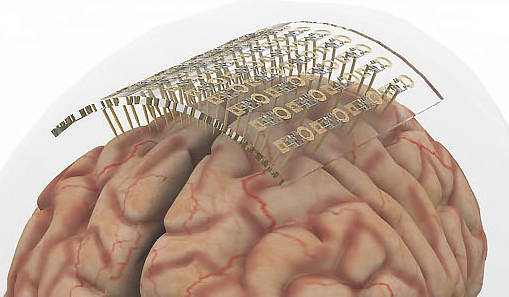
\includegraphics[width=.7\textwidth]{brain_probe.jpg}\\[1em]
%         \begin{columns}
%             \techterm{\color{darkblue} High Localization}%
%             \techterm{Low Resolution}%
%             \techterm{Invasive}%
%         \end{columns}
% }


% \frame[t]{
%     \frametitle{Context: functional Neuroimaging}

%     {\large How to record living brains electrical activity: \textbf{Electrophysiology}}\\[.3em]

%     \large\centering Remote measurement: M/EEG.\\[-.5em]
%     \begin{columns}[T]
%         \column{.35\textwidth}
%         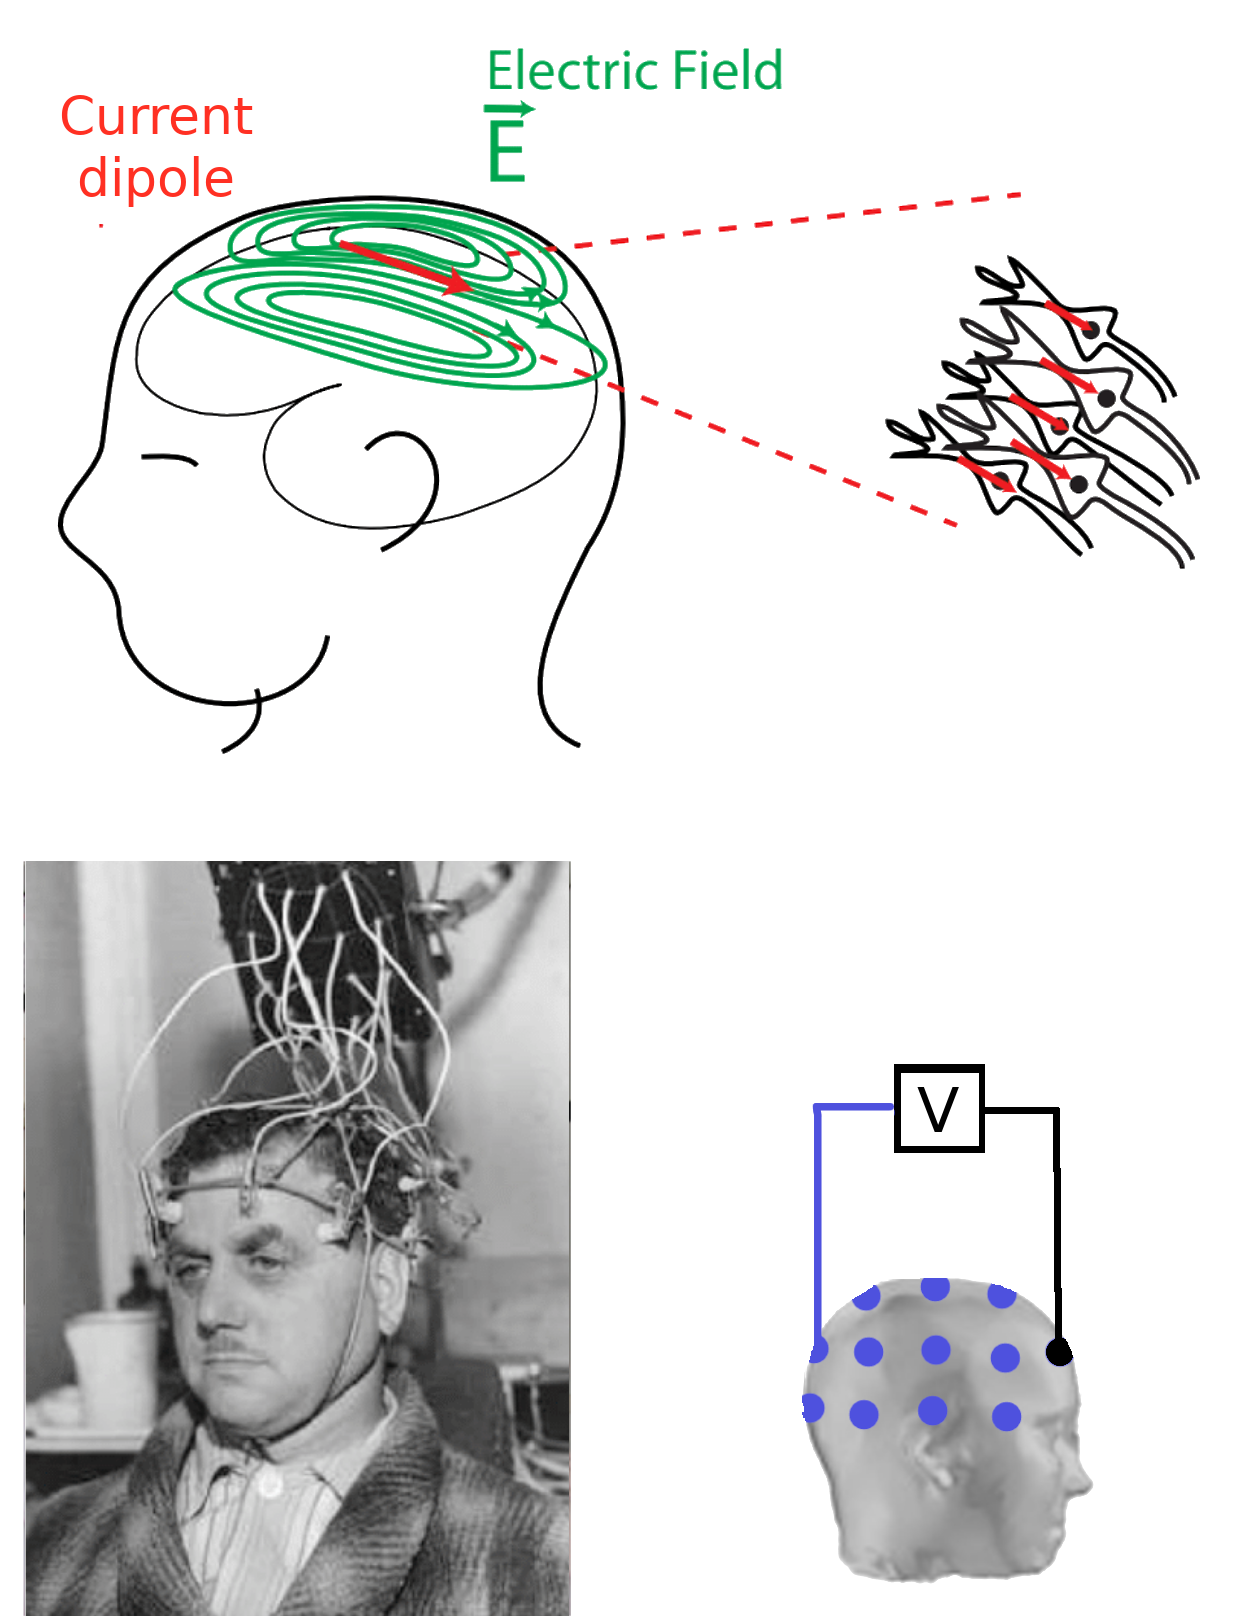
\includegraphics[width=\textwidth]{eeg_presentation}
%         \column{.35\textwidth}
%         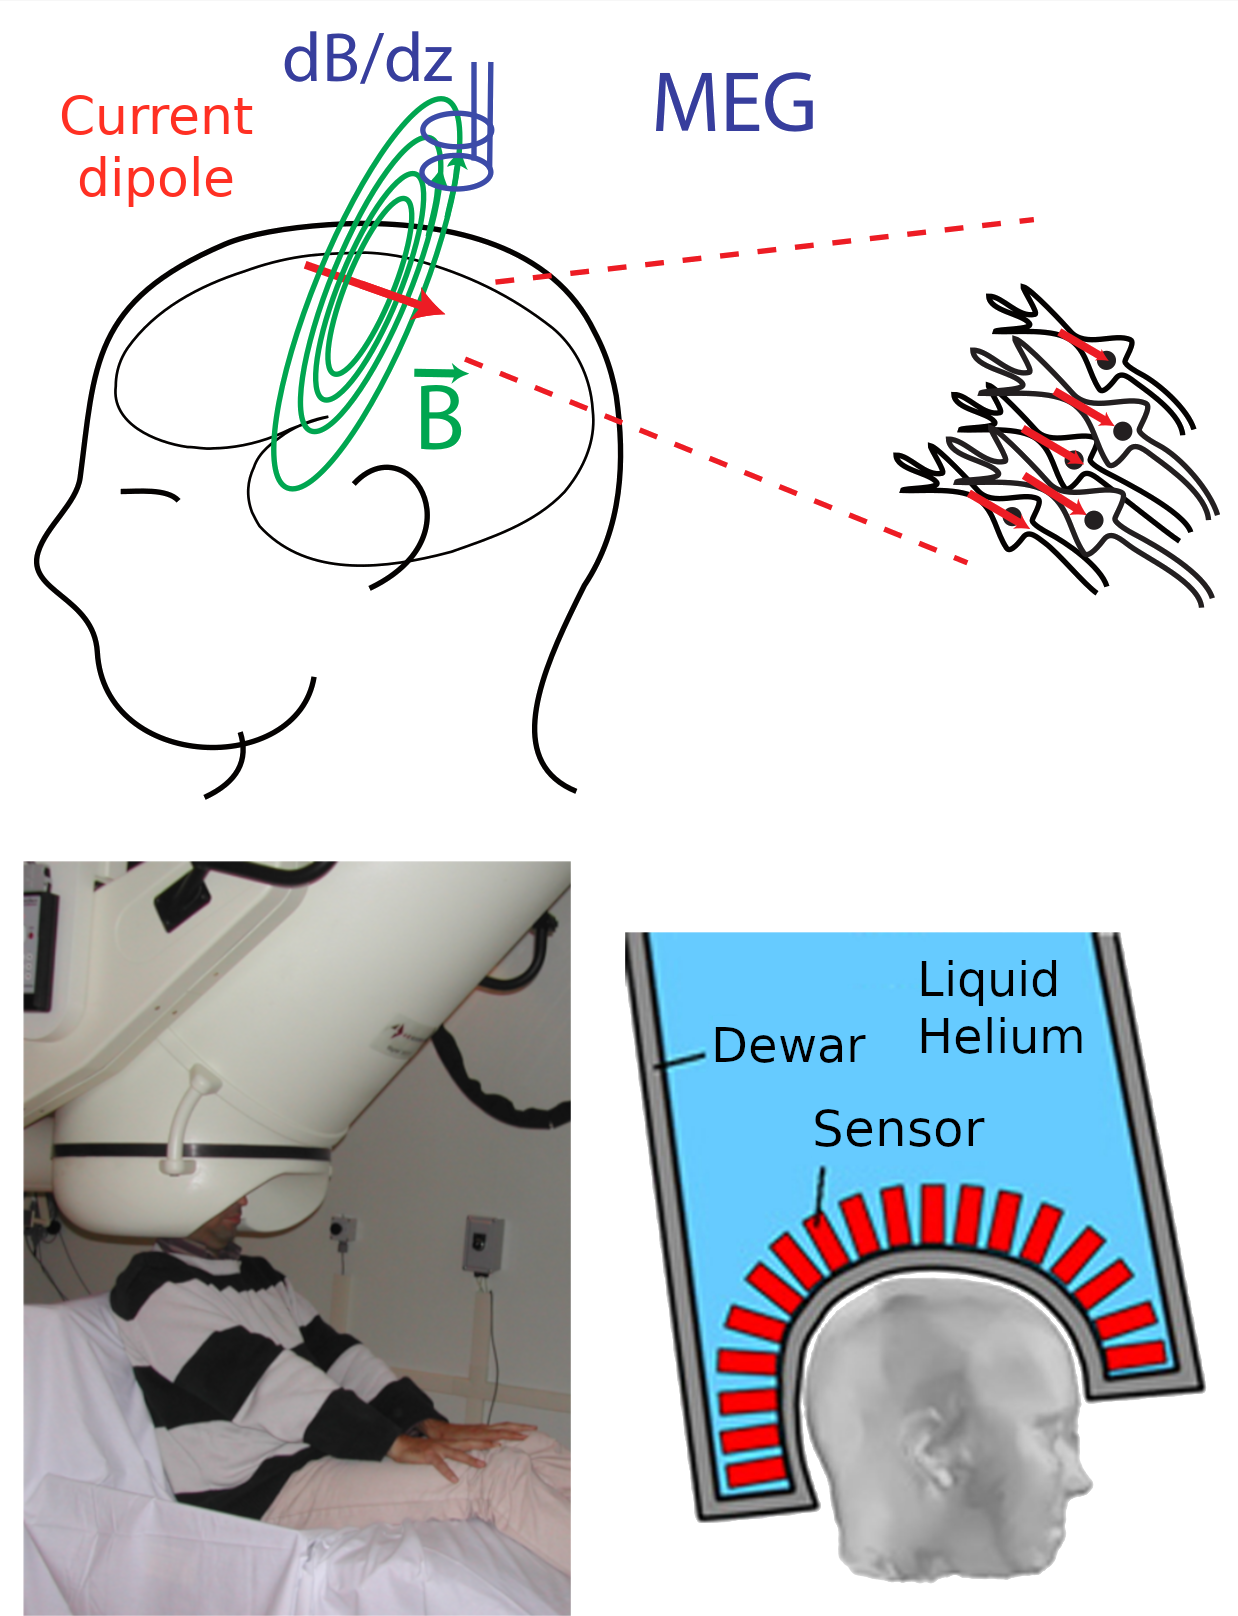
\includegraphics[width=\textwidth]{meg_presentation}
%     \end{columns}
%     % \only<2>{
%     \begin{columns}
%         \techterm{No Localization}%
%         \techterm{\color{darkblue} Global}%
%         \techterm{\color{darkblue} Non Invasive}%
%     \end{columns}
%     % }

% }

% \frame{
%     \frametitle{M/EEG signals}

%     {\Large\bf Multivariate time-series $x$}\\[1em]

%     \centering
%     \alt<3>{
%         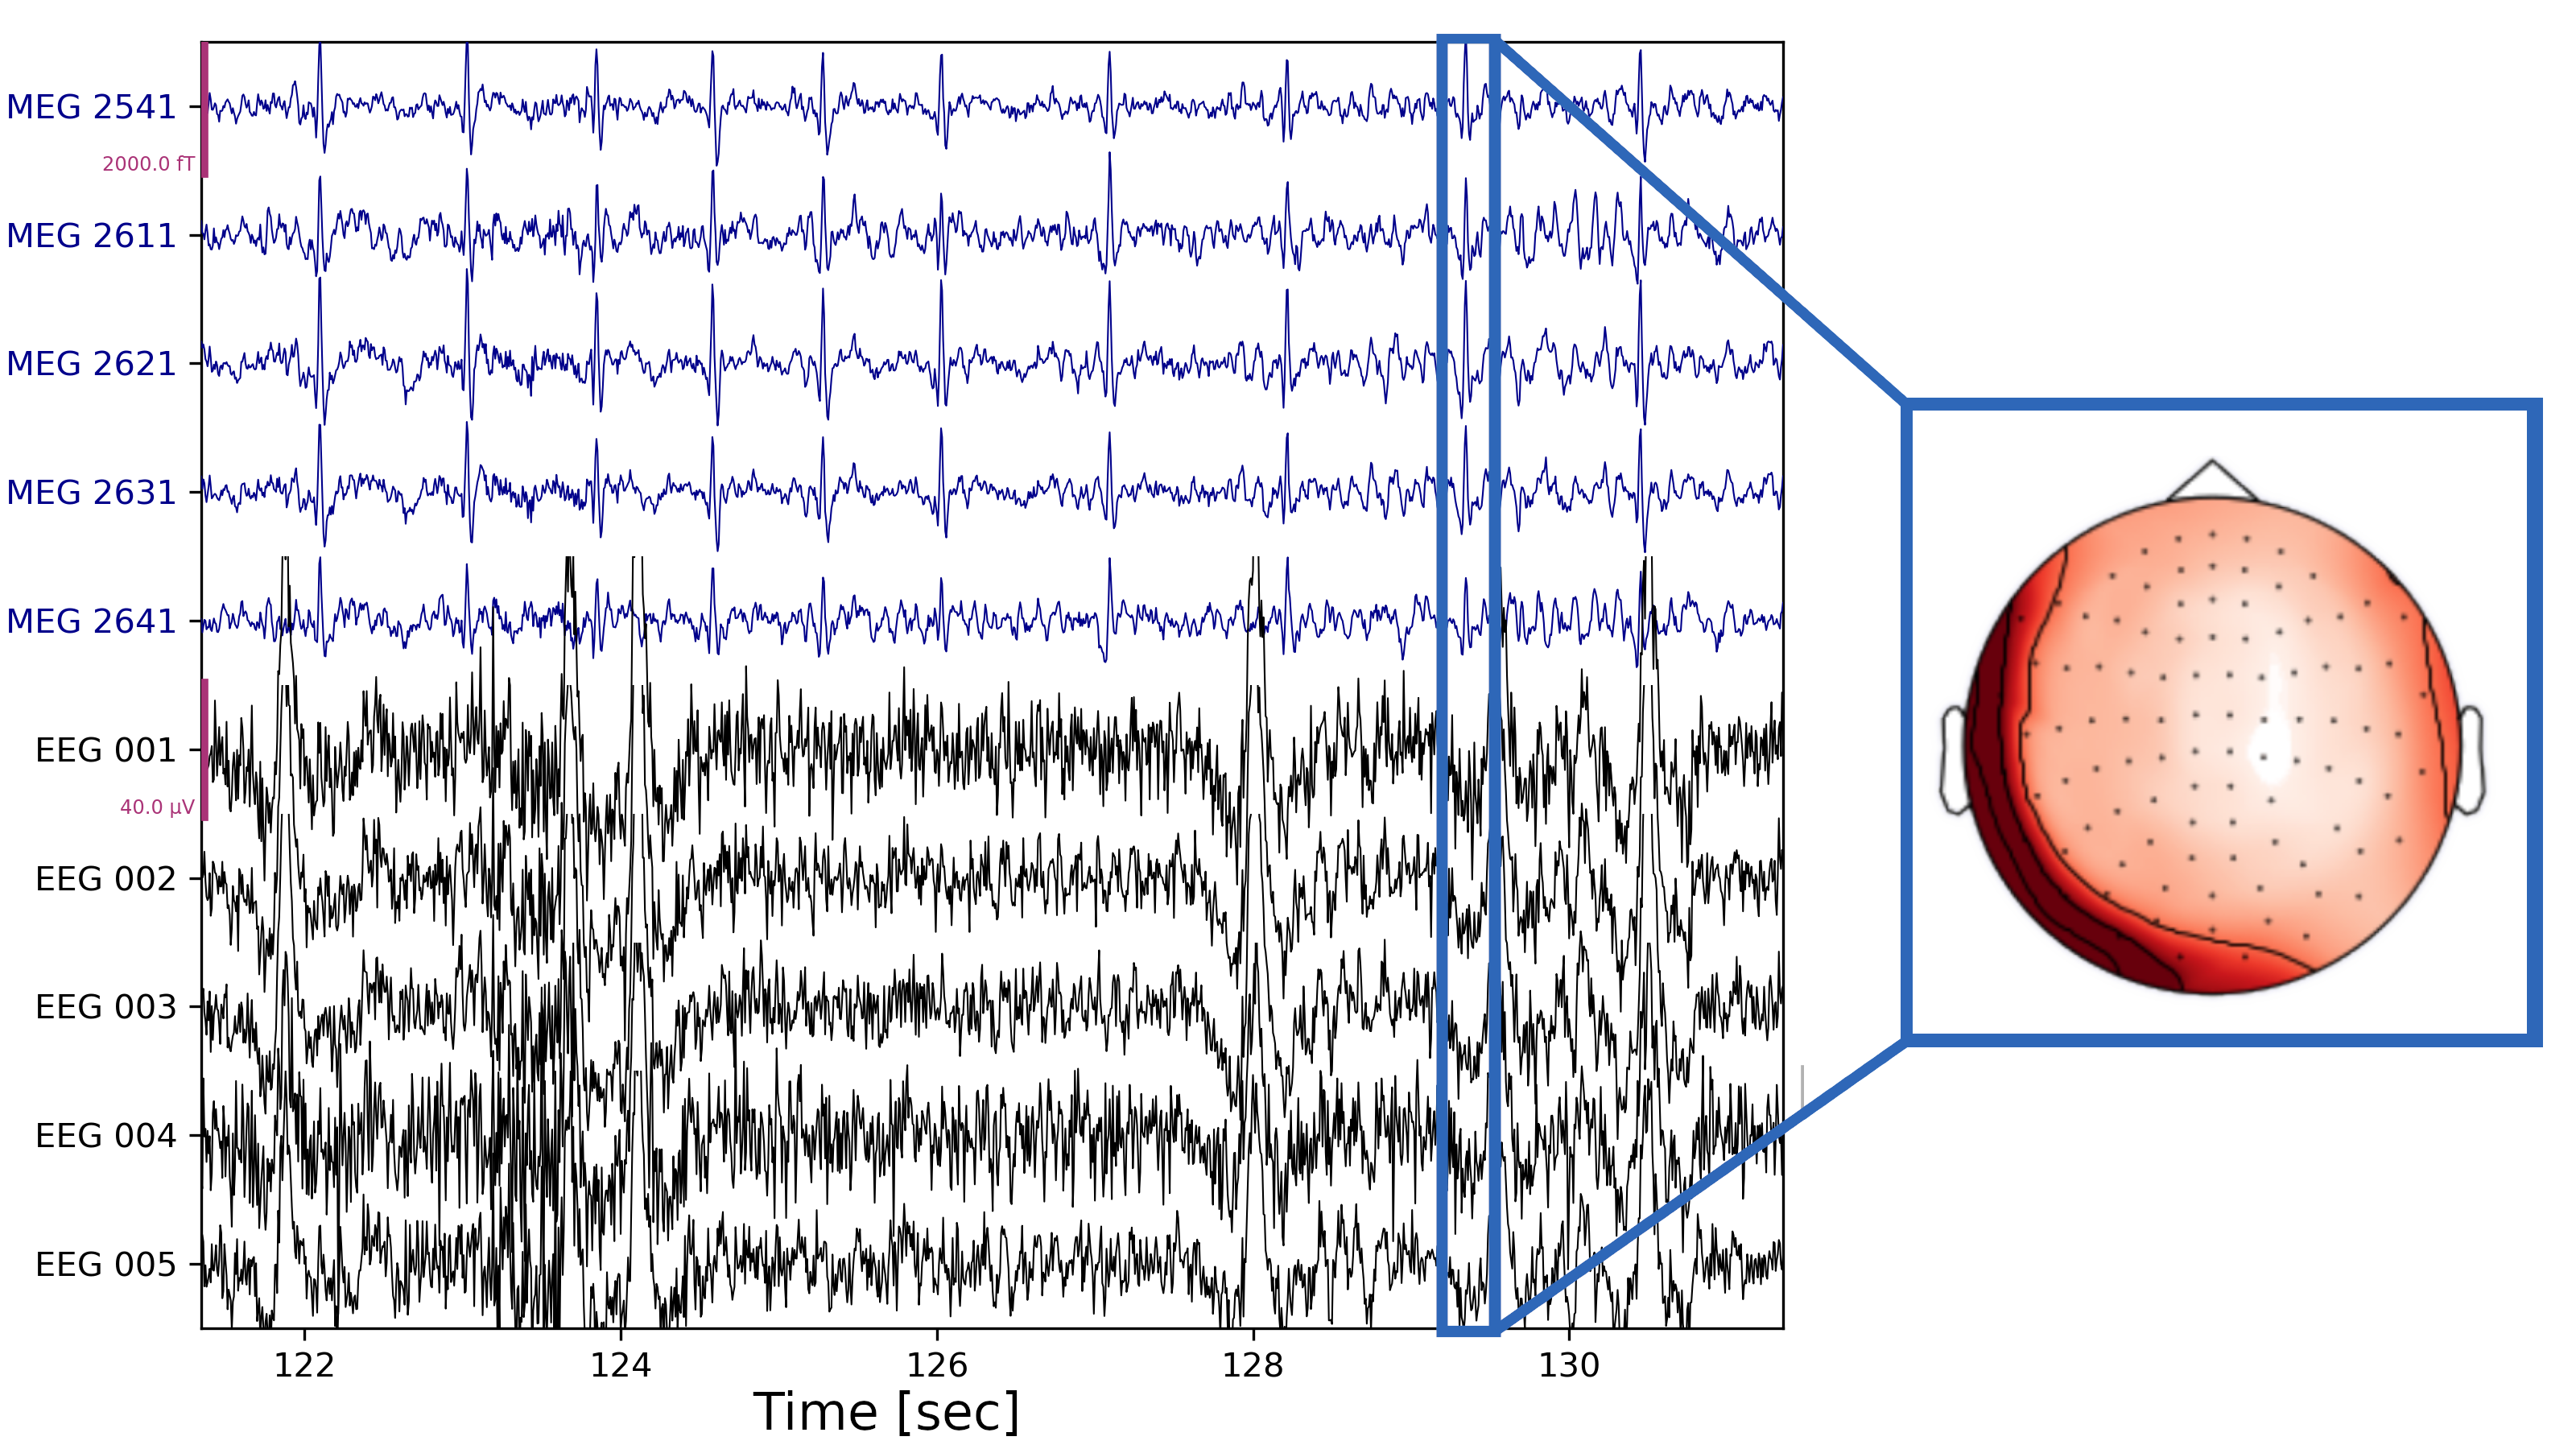
\includegraphics[width=.9\textwidth]{meeg_data_highlight}
%     }{
%         \alt<1>{
%             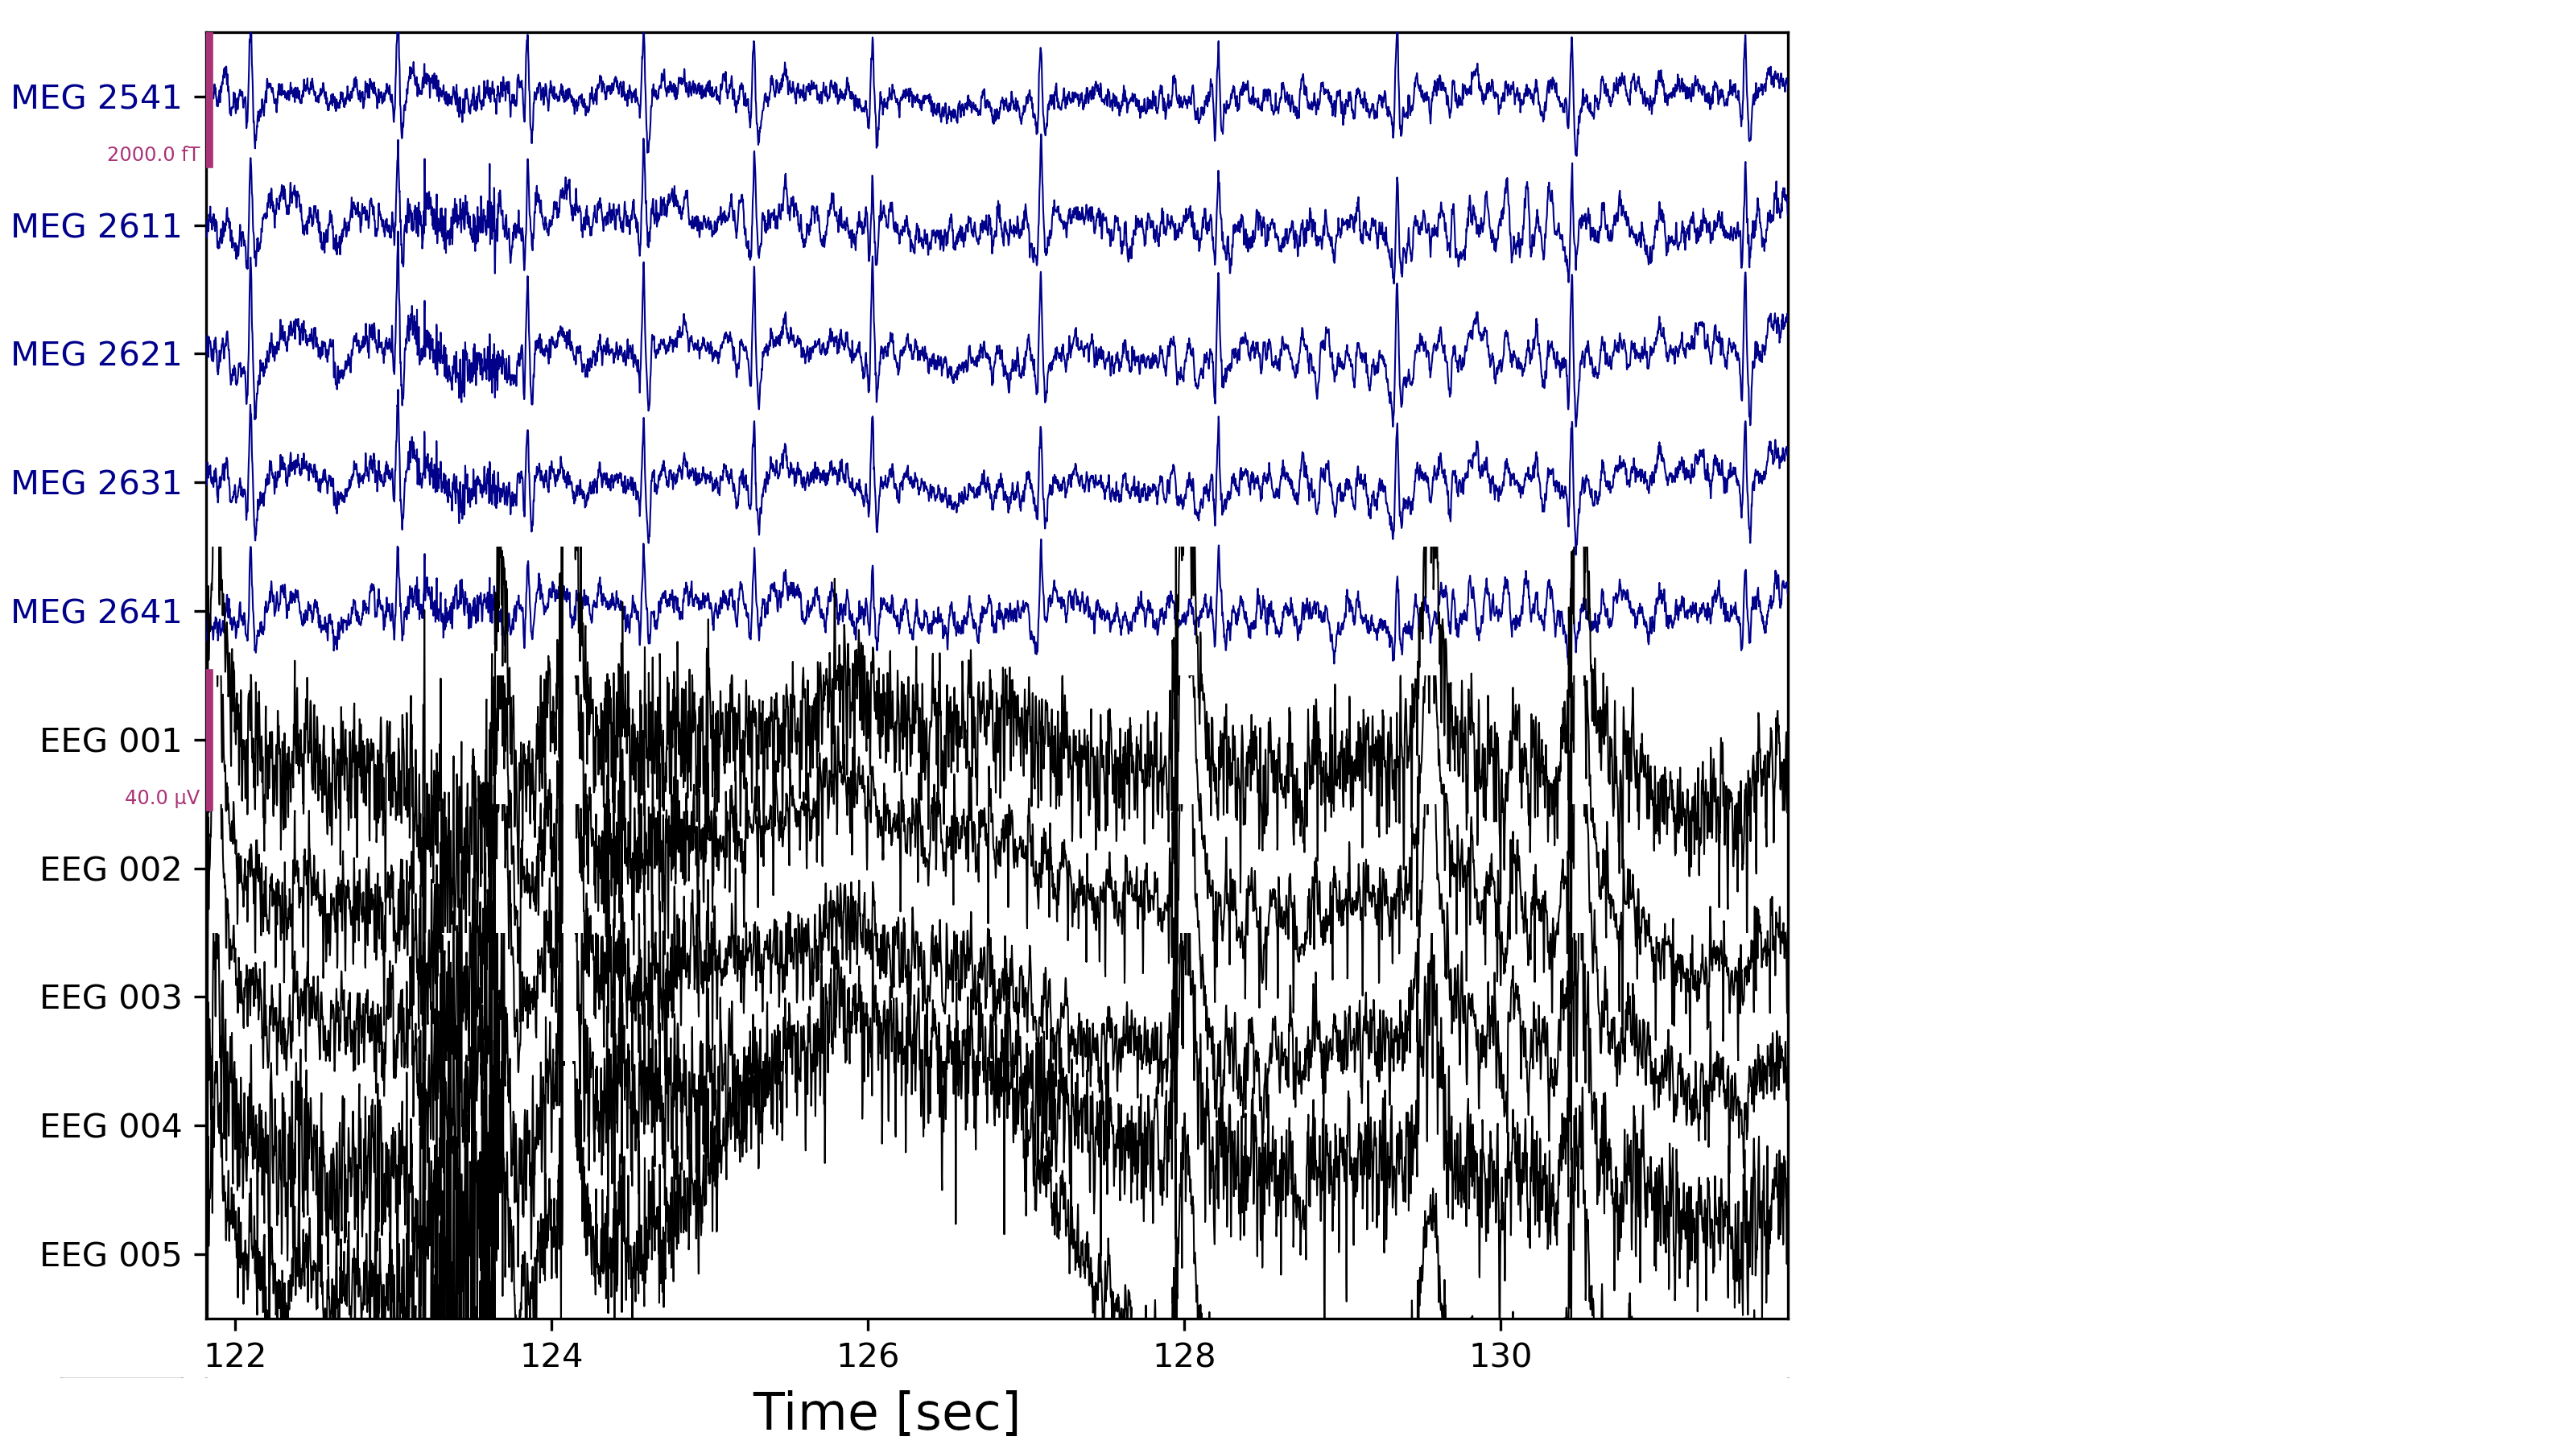
\includegraphics[width=.9\textwidth]{meeg_data}
%         }{
%             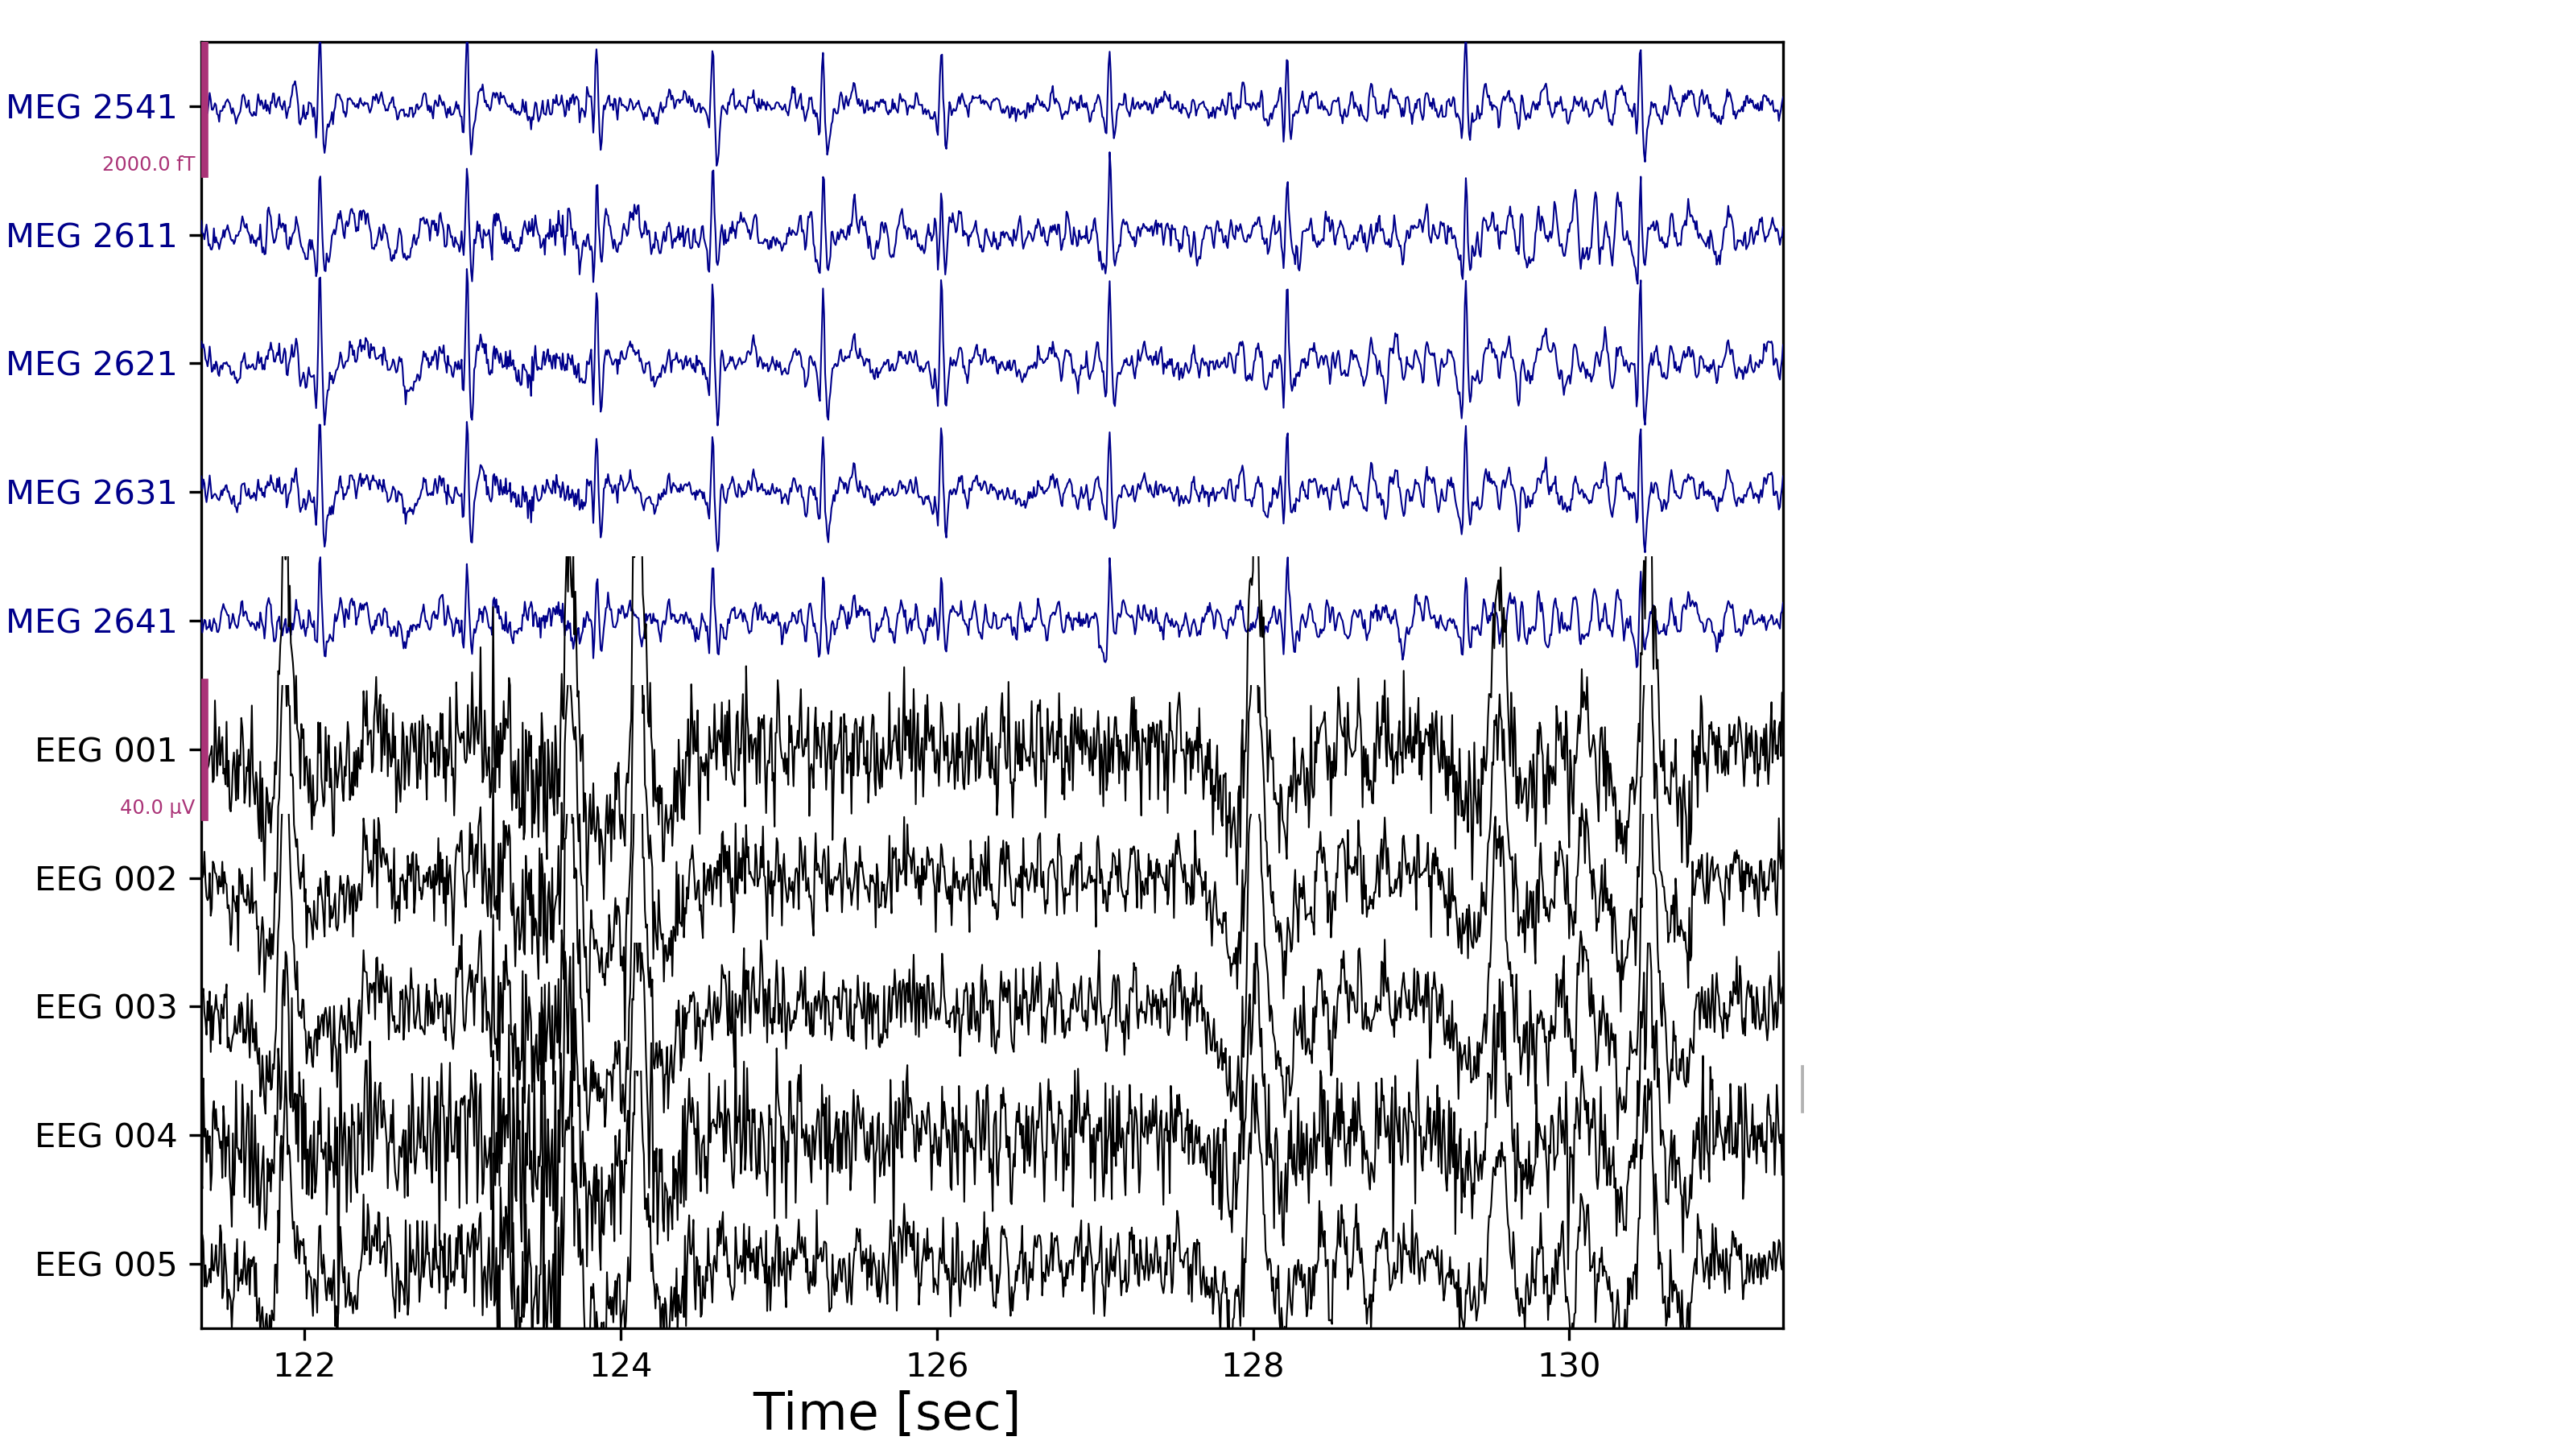
\includegraphics[width=.9\textwidth]{meeg_data_preproc}
%         }
%     }\\[1em]
%     \begin{columns}
%         \techterm{Noisy}%
%         \techterm{Many artifacts}%
%         \techterm{Complex}%
%     \end{columns}
% }

\frame[t]{
    \frametitle{Inverse Problems}


    \nobibliography{library.bib}

    \vskip-1em
    \begin{columns}[T]

        \column{.5\textwidth}
            {\bf Neuroimaging -- M/EEG}\\[.5em]
            {\centering
            \begin{tikzpicture}
            \tikzset{
                %Define standard arrow tip
                >=stealth',
                %Define style for boxes
                varstyle/.style={
                    rectangle,
                    rounded corners,
                    draw=black,
                    text width=1em,
                    minimum height=1.5em,
                    text centered},
                small/.style={
                    font=\footnotesize,
                }
            }
            \node (meg) {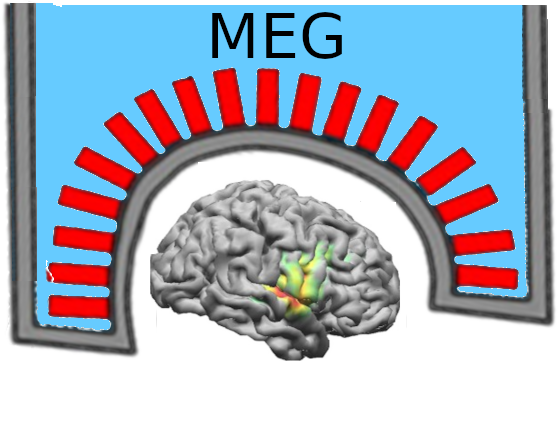
\includegraphics[width=6em]{meg_localised_source}};
            \draw[->, thick] (meg.east) -- ++(6em, 0)
            node[midway, align=center,small] (maxwell) {Maxwell's\\Equations}
            node[right] (topomap) {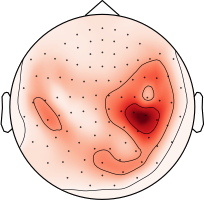
\includegraphics[width=3em]{topomap_somato}};

            \draw[<-, thick] ($(meg.east) + (0, 0.75em)$) to[bend left, looseness=1]
            node [midway, above,small] {Inverse Problem}
            ($(topomap.west) + (0, 0.75em)$);
            \end{tikzpicture}}

            \vskip-.5em
            {\bf Astrophysics}\\[.5em]
            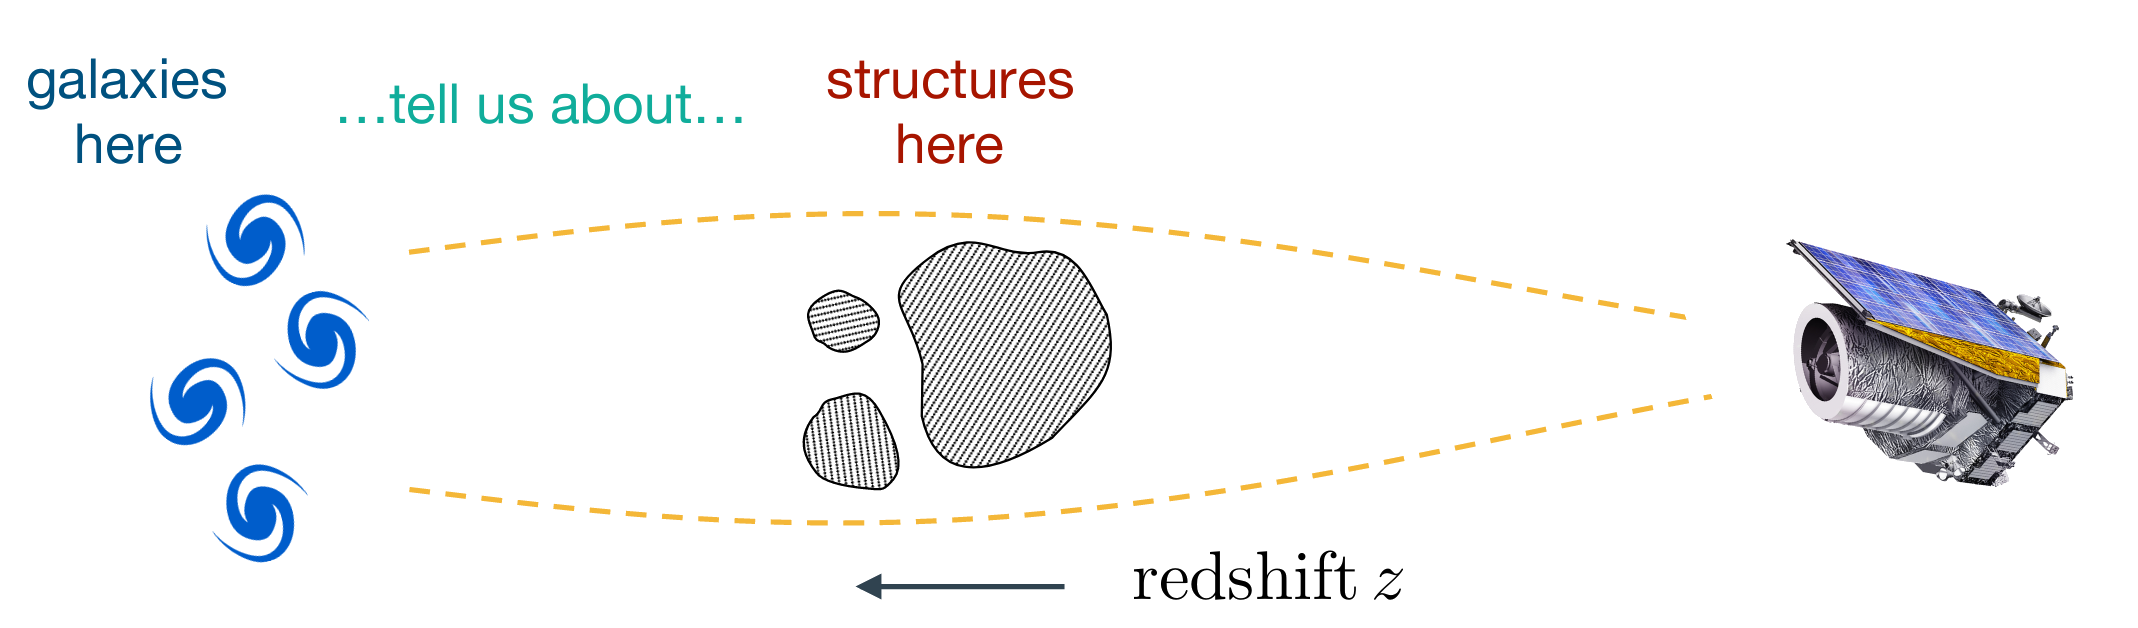
\includegraphics[width=\textwidth]{weak_lensing}\\

            {\bf Seismology -- Prospection}\\[.5em]
            {\centering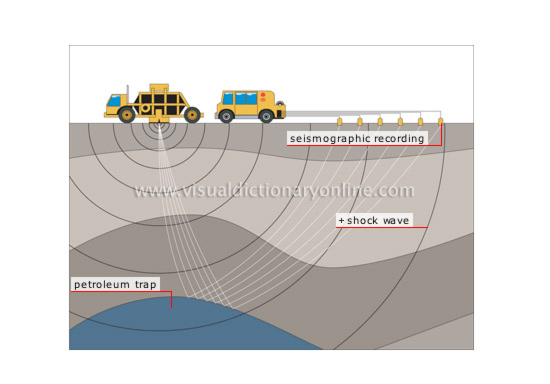
\includegraphics[width=.5\textwidth, trim={6.7em 4em 7em 5em}, clip]{InverseProblem_petroleum}\\}

        \column{.5\textwidth}

            {\bf Neuroimaging -- MRI}\\[1em]
                \begin{columns}[c]
                \column{.5\textwidth}    \centering
                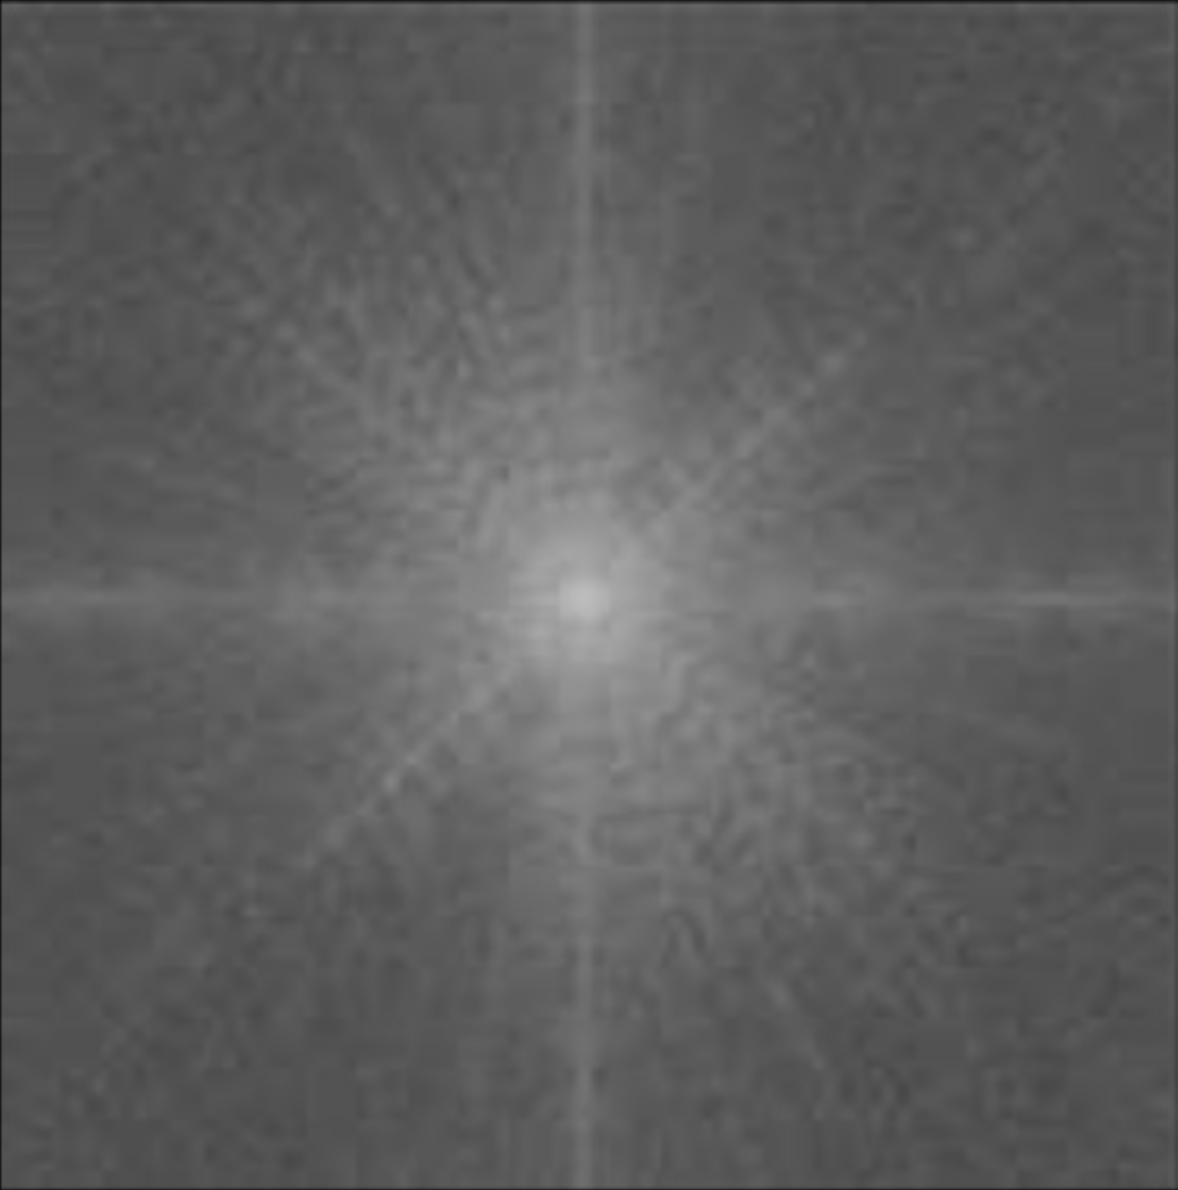
\includegraphics[width=.8\textwidth]{K_space}\\
                \column{.5\textwidth} \centering
                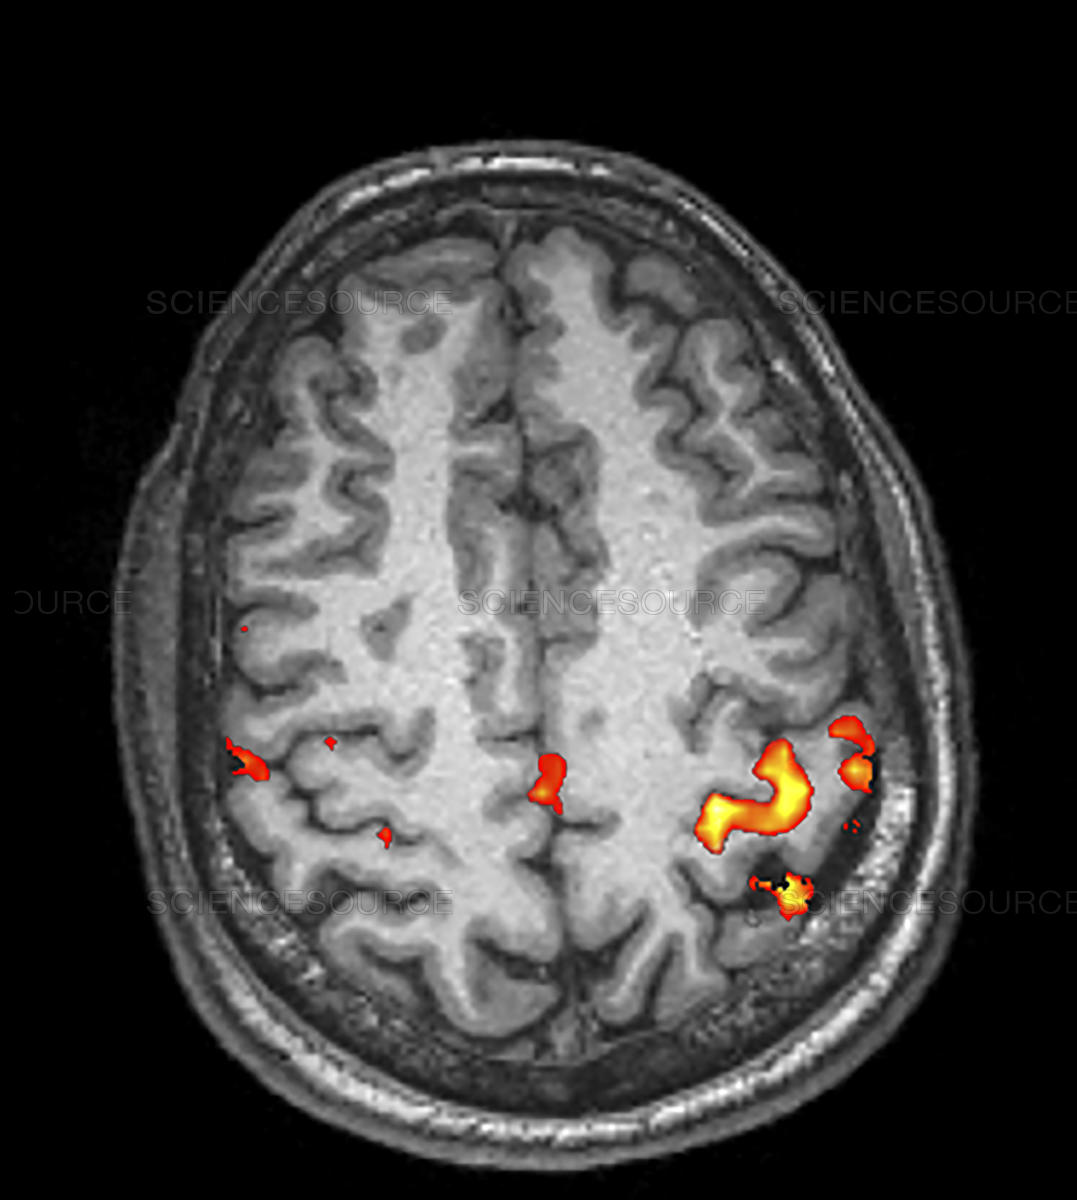
\includegraphics[width=.8\textwidth]{brain_scan}\\
                \end{columns}

            \vskip1.5em
            {\bf Imaging}\\[1em]
            \centering
            \uncovergraphics<1>[width=.8\textwidth, trim={0em 2em 37em 2em}, clip]{super_resolution.png}\\
            Super-Resolution, Inpainting, Deblurring, ...
        \end{columns}

}

\frame{
    \frametitle{Inverse Problem: Source Localization for M/EEG}

    \setbeamercovered{invisible}
    {\centering
    \begin{tikzpicture}
    \tikzset{
        %Define standard arrow tip
        >=stealth',
        %Define style for boxes
        varstyle/.style={
            rectangle,
            rounded corners,
            draw=black,
            text width=1em,
            minimum height=1.5em,
            text centered},
    }
    \node (meg) {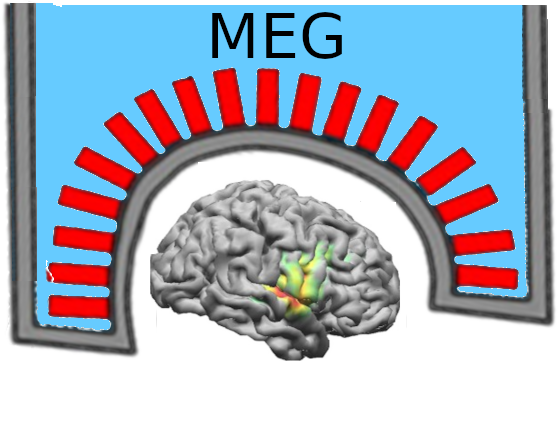
\includegraphics[width=12em]{meg_localised_source}};
    \draw[->, thick] ($(meg.east) - (0, 1.5em)$) -- ++(8em, 0)
    node[midway, align=center] (maxwell) {Maxwell's\\Equations}
    node[right] (topomap) {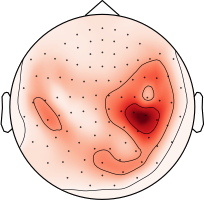
\includegraphics[width=6em]{topomap_somato}};
    \node[varstyle, below=.5em] at (topomap.south) (varX) {$\varX$};
    \node[below=0em of varX.south] {\bf Observed signal};
%        \draw[->, thick] (topomap.east) -- ++(5em, 0)
%        node[midway, align=center] {\small Problème\\ \small inverse}
    \node[varstyle, below=.2em of meg]
        (varZ) {$\varZ$};
        \node[below=0em of varZ.south] {\bf Electrical activity};
    \node[varstyle, below=3.8em of maxwell.center]
        (varD) {$\varD$};

    {
         \draw[<-, thick] (meg.east) to[bend left, looseness=1]
            node [midway, above] {Inverse Problem}
            ($(topomap.west) + (0, 1.5em)$);
    }
    \end{tikzpicture}}
    \vskip0em
    {\bf Forward model: }$\varX{} = \varD\varZ + \varepsilon$
    \hskip3em
    {{\bf Inverse problem:} find $\varZ$ from $\varX$}\\
    {
        \vskip1em
        \myitem{} Noisy problem: need to account for $\varepsilon$\\[.5em]
        \myitem{} Ill-posed problem: many solutions $\varZ$ such that $\varD\varZ=\varX$,\\\quad\quad need to select one.
    }

}

% \frame[t]{
%     \frametitle{Inverse Problems}

%     \vskip-1em
%     \begin{columns}[T]

%         \column{.5\textwidth}
%             {\bf Neuroimaging -- M/EEG}\\[.5em]
%             {\centering
%             \begin{tikzpicture}
%             \tikzset{
%                 %Define standard arrow tip
%                 >=stealth',
%                 %Define style for boxes
%                 varstyle/.style={
%                     rectangle,
%                     rounded corners,
%                     draw=black,
%                     text width=1em,
%                     minimum height=1.5em,
%                     text centered},
%                 small/.style={
%                     font=\footnotesize,
%                 }
%             }
%             \node (meg) {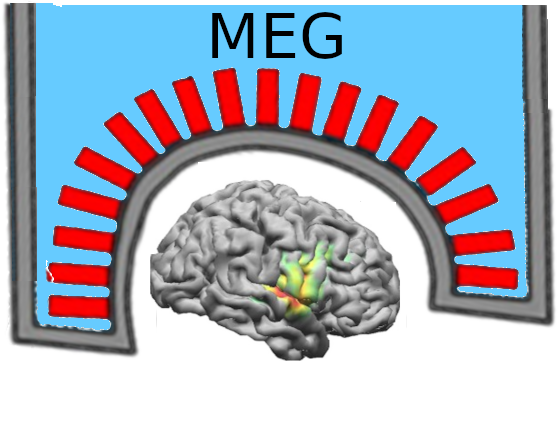
\includegraphics[width=6em]{meg_localised_source}};
%             \draw[->, thick] (meg.east) -- ++(6em, 0)
%             node[midway, align=center,small] (maxwell) {Maxwell's\\Equations}
%             node[right] (topomap) {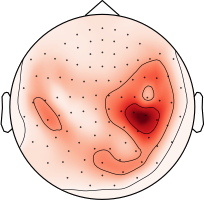
\includegraphics[width=3em]{topomap_somato}};

%             \draw[<-, thick] ($(meg.east) + (0, 0.75em)$) to[bend left, looseness=1]
%             node [midway, above,small] {Inverse Problem}
%             ($(topomap.west) + (0, 0.75em)$);
%             \end{tikzpicture}}

%             \vskip-.5em
%             {\bf Astrophysics}\\[.5em]
%             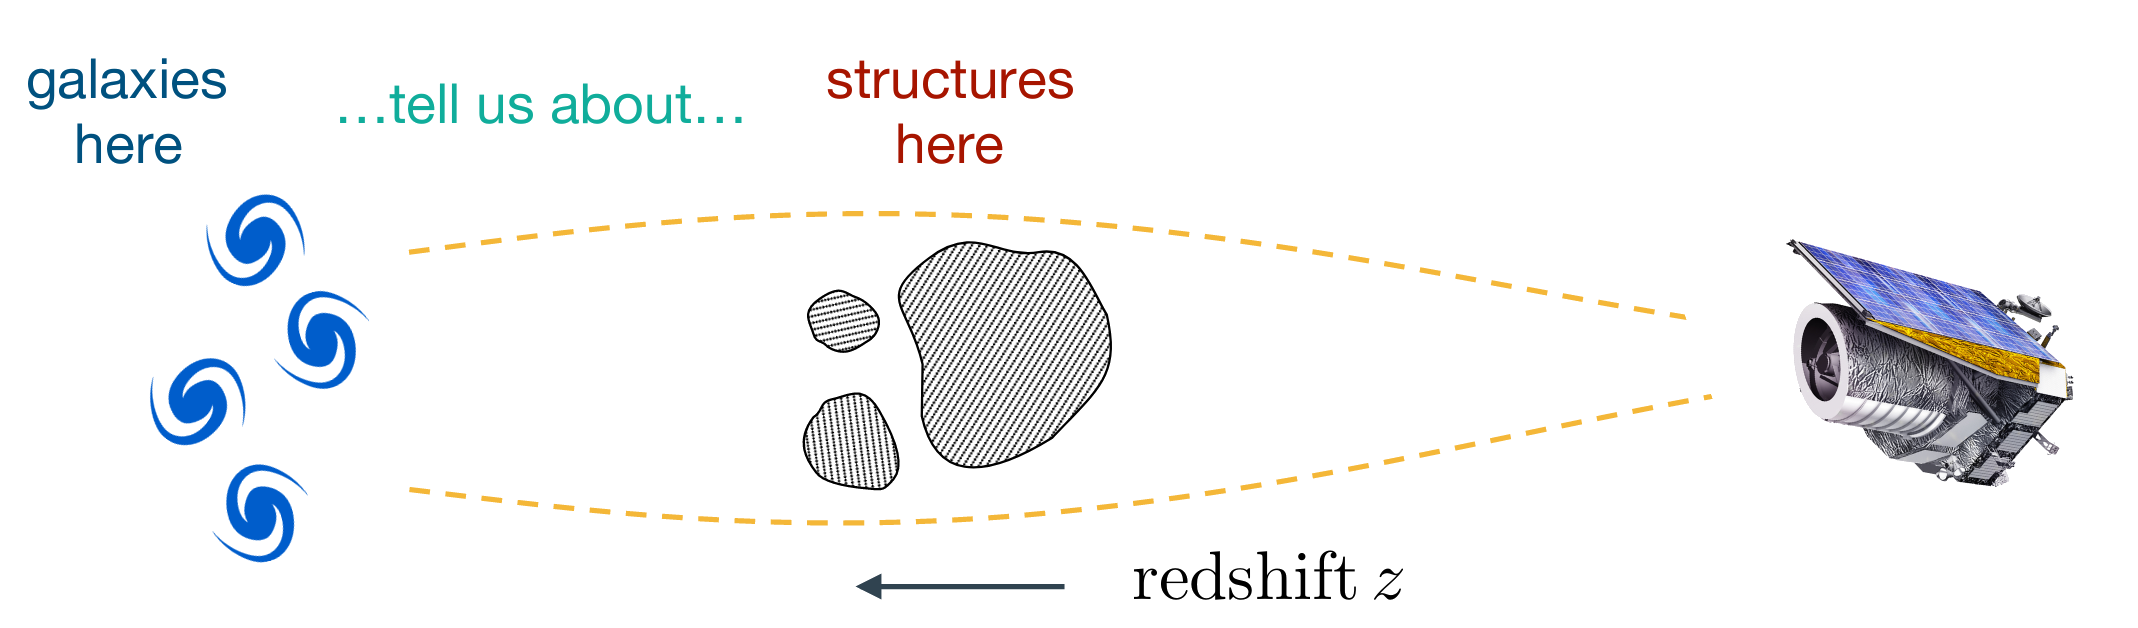
\includegraphics[width=\textwidth]{weak_lensing}\\

%             {\bf Seismology -- Prospection}\\[.5em]
%             {\centering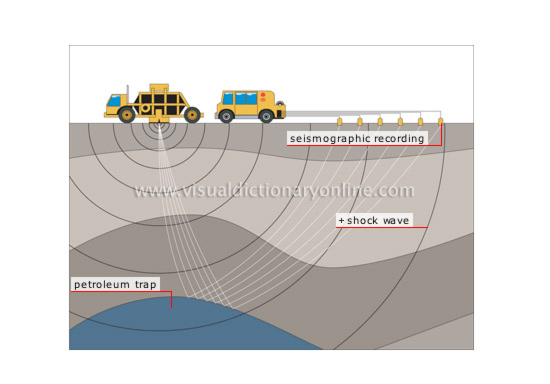
\includegraphics[width=.5\textwidth, trim={6.7em 4em 7em 5em}, clip]{InverseProblem_petroleum}\\}

%         \column{.5\textwidth}

%             {\bf Neuroimaging -- MRI}\\[1em]
%                 \begin{columns}[c]
%                 \column{.5\textwidth}    \centering
%                 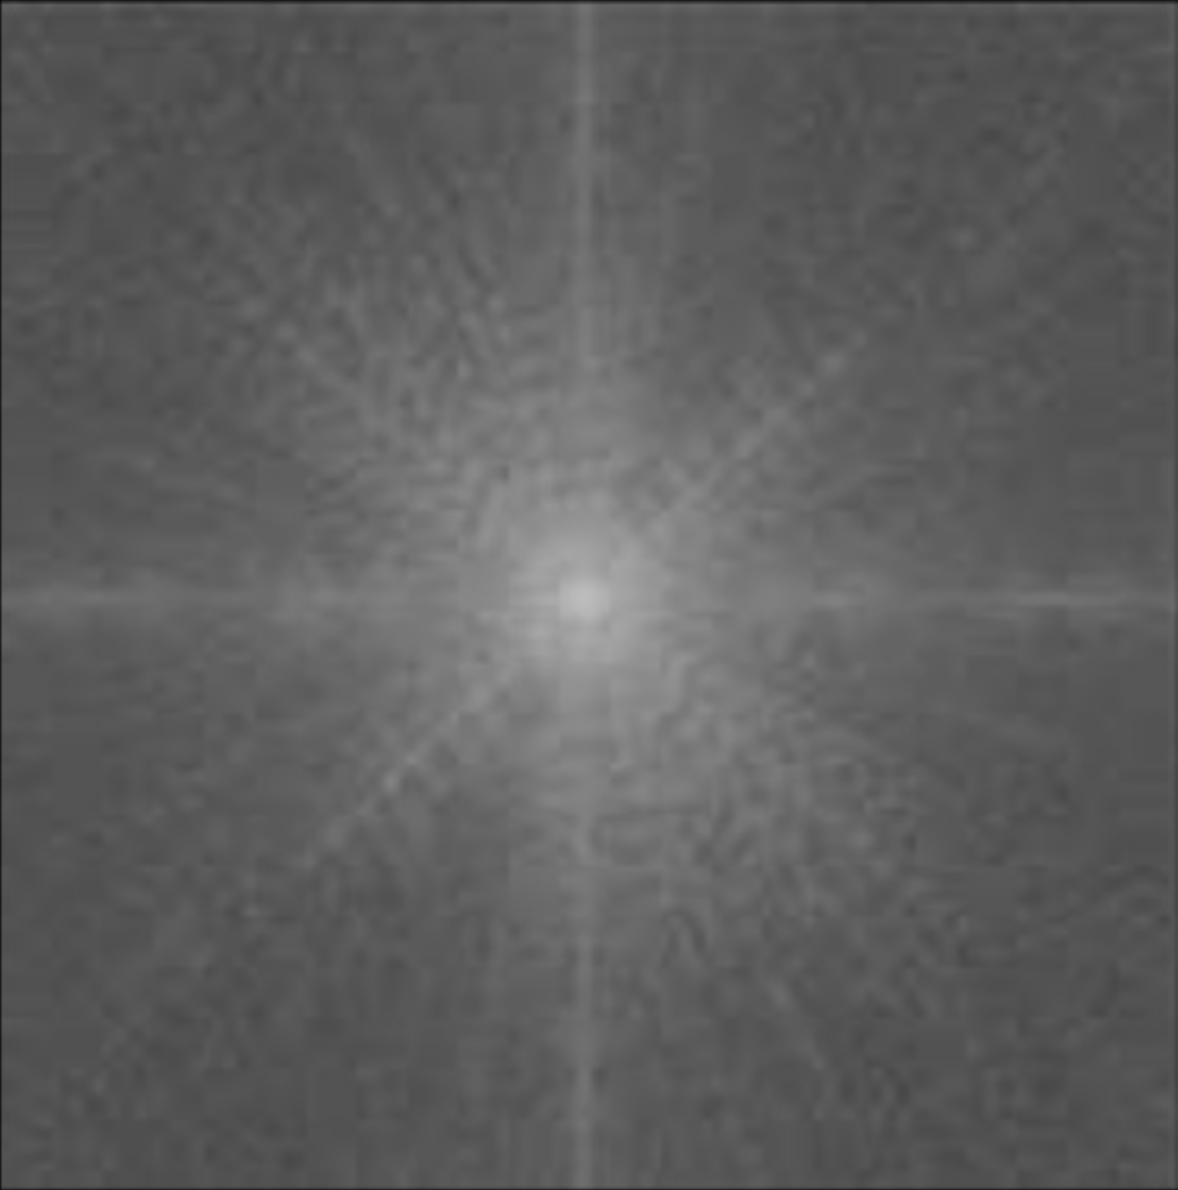
\includegraphics[width=.8\textwidth]{K_space}\\
%                 \column{.5\textwidth} \centering
%                 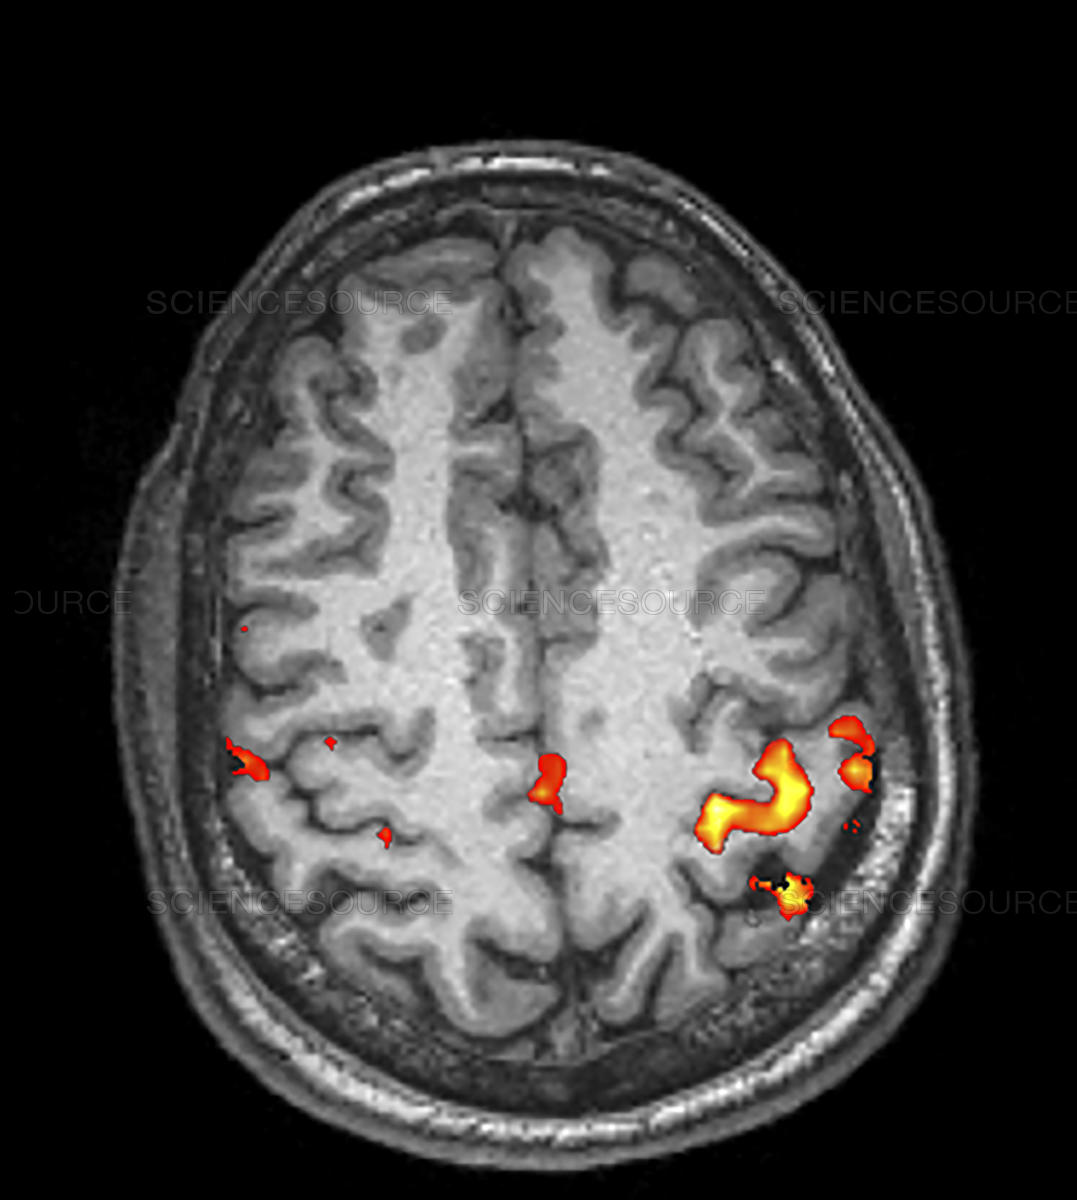
\includegraphics[width=.8\textwidth]{brain_scan}\\
%                 \end{columns}

%             \vskip1.5em
%             {\bf Imaging}\\[1em]
%             \centering
%             \uncovergraphics<1>[width=.8\textwidth, trim={0em 2em 37em 2em}, clip]{super_resolution.png}\\
%             Super-Resolution, Inpainting, Deblurring, ...
%         \end{columns}

%         \vskip-13em
%         {\centering\highlight{
%             \parbox{.7\textwidth}{
%                 \vskip1em\centering
%                 For many inverse problems, we don't have access to
%                 large training sets with pairs $(\varX, \varZ)$.
%                 \vskip1em
%             }
%         }\\}
% }




\frame[t]{
    \frametitle{Inverse Problem Resolution}
    {\bf MAP estimate as a regularized regression problem}\\[.5em]

    \[
        \varZ^*(\varX; \theta) = \argmin_\varZ \underbrace{\frac12\|\varX - \varD\varZ\|_2^2}_{-log~p(\varX| \varZ)} ~+ \underbrace{\mathcal R(\varZ{}; \theta)}_{-log~p(\varZ; \theta)}
    \]
    where $\mathcal R$ encodes prior information to select a good/plausible solution.\\[2em]

    \pause{}
    \underline{\bf Common framework:}
    \begin{itemize}
        \item \textbf{Efficient solvers:} Forward backward, ADMM,  \dots\\
        \strongpoint{But might require many iterations to get quality estimate.}
        \item[]
        \item \textbf{Flexible:} Can choose many priors -- \emph{handpicked, learned, implicit, \dots}
    \end{itemize}

    \strongpoint{
        Quality of the solution depends on the prior's choice
        $p(\varZ; \theta)$
    }
}

\frame{
    \frametitle{Prior learning as a bilevel problem}

    Evaluate the quality of a solution with $\mathcal L$, and try to find the best prior:\\[1em]
    \[
        \min_\theta \mathcal L(\varZ^*(\varX; \theta))
        \quad s.t. \quad \varZ^*(\varX; \theta) = \argmin \underbrace{-log~p(\varZ | \varX; \theta)}_{F(\varZ, \theta)}
    \]

    \vskip.5em
    \pause{}
    \textbf{How to solve such problem:}\\[1em]
    \begin{itemize}
        \item \emph{Random search:} sample some $\theta$ and keep the "best one".
        \strongpoint{Slow for $\theta$ in high dimension.}\vskip.5em
        \item \emph{Gradient based method:} use first order information:
        \begin{align*}
            \frac{d\mathcal L(\varZ^*(\varX; \theta))}{d \theta} & =  \frac{d\varZ^*(\varX; \theta)}{d \theta}^\top\frac{\partial \mathcal L}{\partial z} (\varZ^*(\varX; \theta))
        \end{align*}
        \strongpoint{Expensive to compute $\varZ^*(\varX; \theta)$ and its Jacobian.}
    \end{itemize}
}

\frame[t]{
    \frametitle{Unrolling for prior learning}

    \textbf{Idea:}\vskip1em
    \begin{itemize}
        \item Replace $\varZ^*(\varX; \theta)$ by $\varZ^N(\varX; \theta, \psi)$ with hyperparameter $\psi$.\\[.5em]
        \item Compute the Jacobian using backpropagation through the network.
    \end{itemize}

    \pause{}
    \strongpoint{\bf Why?}
    \vskip1em
    \alt<3->{
        \textbf{Learned solver:} To solve with many $\varX$ and a single $\varD$, learn $\psi$\\[.5em]
        \begin{itemize}
            \item Learning algorithm to resolve the original problem faster.
            \item With supervised or unsupervised losses.
        \end{itemize}
    }{
        \textbf{Prior learning:} learn $\theta$ to get the prior that gives the best reconstruction.\\[.5em]
        \begin{itemize}
            \item \emph{Supervised:} $\mathcal L(\theta) = \mathbb E_{(\varX, \varZ)}\frac12\|\varZ - \varZ^N(\varX; \theta, \psi)\|_2^2$\\[.5em]
            \item \emph{Unsupervised:} consistency loss, \dots\\[.5em]
        \end{itemize}
    }
    \visible<4>{
        \vskip1em
        \strongpoint{
            What can we say about the learned procedure?\\
            Convergence toward $\varZ^*(\varX; \theta)$?
        }
    }
}

\frame{
    \frametitle{Unrolling for prior learning}

    {\centering
    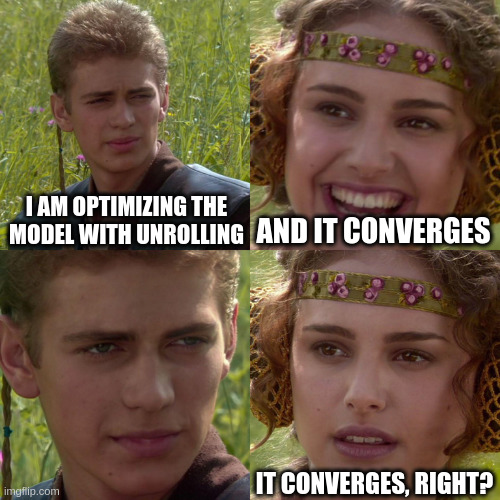
\includegraphics[width=.6\textwidth]{anakin.jpg}\\}
}


\begin{comment}

\begin{frame}[t]{Iterative Shrinkage-Thresholding Algorithm \mycite{Daubechies2004}}
    Proximal gradient descent algorithm with $\mathcal R(\varZ) = \lambda\|\varZ\|_1$,
    \alt<1>{\[
        z^{(t+1)} = st\left(z^{(t)}
                                   - \alpha\underbrace{\nabla f_x(z^{(t)})}_{G^\top(G z^{(t)} - x)},
                                   \alpha\lambda\right)
    \]}{\[
        z^{(t+1)} = st\left(
            \textcolor{linkcolor}{(Id - \alpha G^\top G)} z^{(t)}
            + \textcolor{D}{\alpha G^\top} x,
            \textcolor{Z}{\alpha\lambda}
        \right)
    \]}
    where $\alpha$ is a step size taken in $[0, \frac{2}{\|G\|_2^2}]$.\\[1em]

    \only<1>{
        \begin{columns}[T]
            \column{.48\textwidth}

            $st$ is the soft-thresholding operator.\\[2em]
            \myitem{} Proximal operator for $\ell_1$-norm.\\[1em]
            \myitem{} Push for sparse vector.
            \column{.5\textwidth}
            \vskip-1em
            \centering
                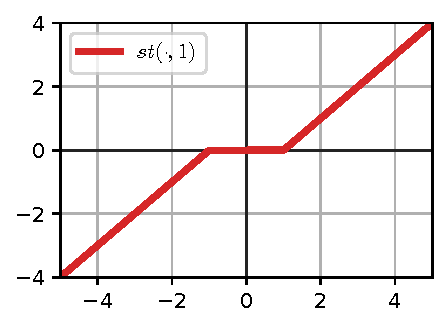
\includegraphics[width=.8\textwidth]{soft_thresholding}\\
        \end{columns}
    }
    \only<2->{
        \begin{columns}
            \column{.55\textwidth}
                {\bf Computational graph interpretation:}\\[1em]
                \myitem{} $W_z = \textcolor{linkcolor}{Id - \alpha G^\top G}$\\[.5em]
                \myitem{} $W_X = \textcolor{D}{\alpha G^\top} $
                \hskip2ex\myitem{} $\beta=\textcolor{Z}{\alpha\lambda}$
            \column{.45\textwidth}
            \vskip2em
            \inputTikZ{.8}{one_step_ista.tex}
        \end{columns}
    }
\end{frame}

\frame[t]{
    \frametitle{Learned ISTA \mycite{Gregor2010}}

    {\bf \alt<2->{Learned}{Unrolled} ISTA:\\[1em]}
    {\centering\alt<2->{
        \inputTikZ{.8}{lista_tikz.tex}
    }{
        \inputTikZ{.8}{ista_unrolled}
    }\\[1em]}

    \only<1>{
        Equivalent to ISTA with $W_z = Id - \alpha G^\top G$, $W_X = \alpha G^\top $ and $\beta = \alpha\lambda$.\\[1em]

        \only<1>{\centering 3 iterations of ISTA $\Leftrightarrow$ 3 layers in the neural network\\}
    }

    % \only<2>{
    %     \vskip2em
    %     If the number of layer goes to infinity, ISTA is equivalent to the RNN:\\[1em]
    %     \begin{columns}
    %         \column{.5\textwidth}
    %         {\centering\inputTikZ{.8}{ista_tikz.tex}\\}
    %         \column{.5\textwidth}
    %         {\bf Implicit deep learning (DEQs):\\[.5em]}
    %         $z^* = st(W_z z^* + W_X x, \beta)$
    %     \end{columns}
    % }

    % \only<2->{

    %     \begin{columns}[T]
    %         \column{.42\textwidth}
    %             \highlight{\parbox{\textwidth}{
    %                 {\bf Supervised}\\[.5em]\color{black}\normalsize\normalfont
    %                 Access to the ground truth $z$:
    %                 \[
    %                     \min_\Theta\mathbb E_{x,z}\Big[\frac12\|z - \Phi_\Theta(x) \|_2^2\Big]
    %                 \]
    %             }}

    %         \column{.52\textwidth}

    %         \highlight{\parbox{\textwidth}{
    %         {\bf Unsupervised}\\[.5em]\color{black}\normalsize\normalfont
    %         No ground truth:
    %         \[
    %             \min_\Theta\mathbb E_{x}\Big[\frac12\|x - G\Phi_\Theta(x) \|_2^2 + \lambda \|\Phi_\Theta(x)\|_1\Big]
    %         \]
    %         }}
    %     \end{columns}
    % }
    \only<2>{
        \begin{columns}[c]
            \column{.55\textwidth}
            Learn
        $\Theta = (W_X^{(t)}, W_z^{(t)}, \beta^{(t)})_{t=0}^T$ s.t.
            \[
                F_x(\Phi_\Theta(x)) \le F_x(ISTA_N(x))
            \]
            {\bf Goal:}
            \strongpoint{Find the same solution as ISTA!}
            \vskip-.5em
            \strongpoint{Faster?}

            \column{.45\textwidth}
            {\centering
            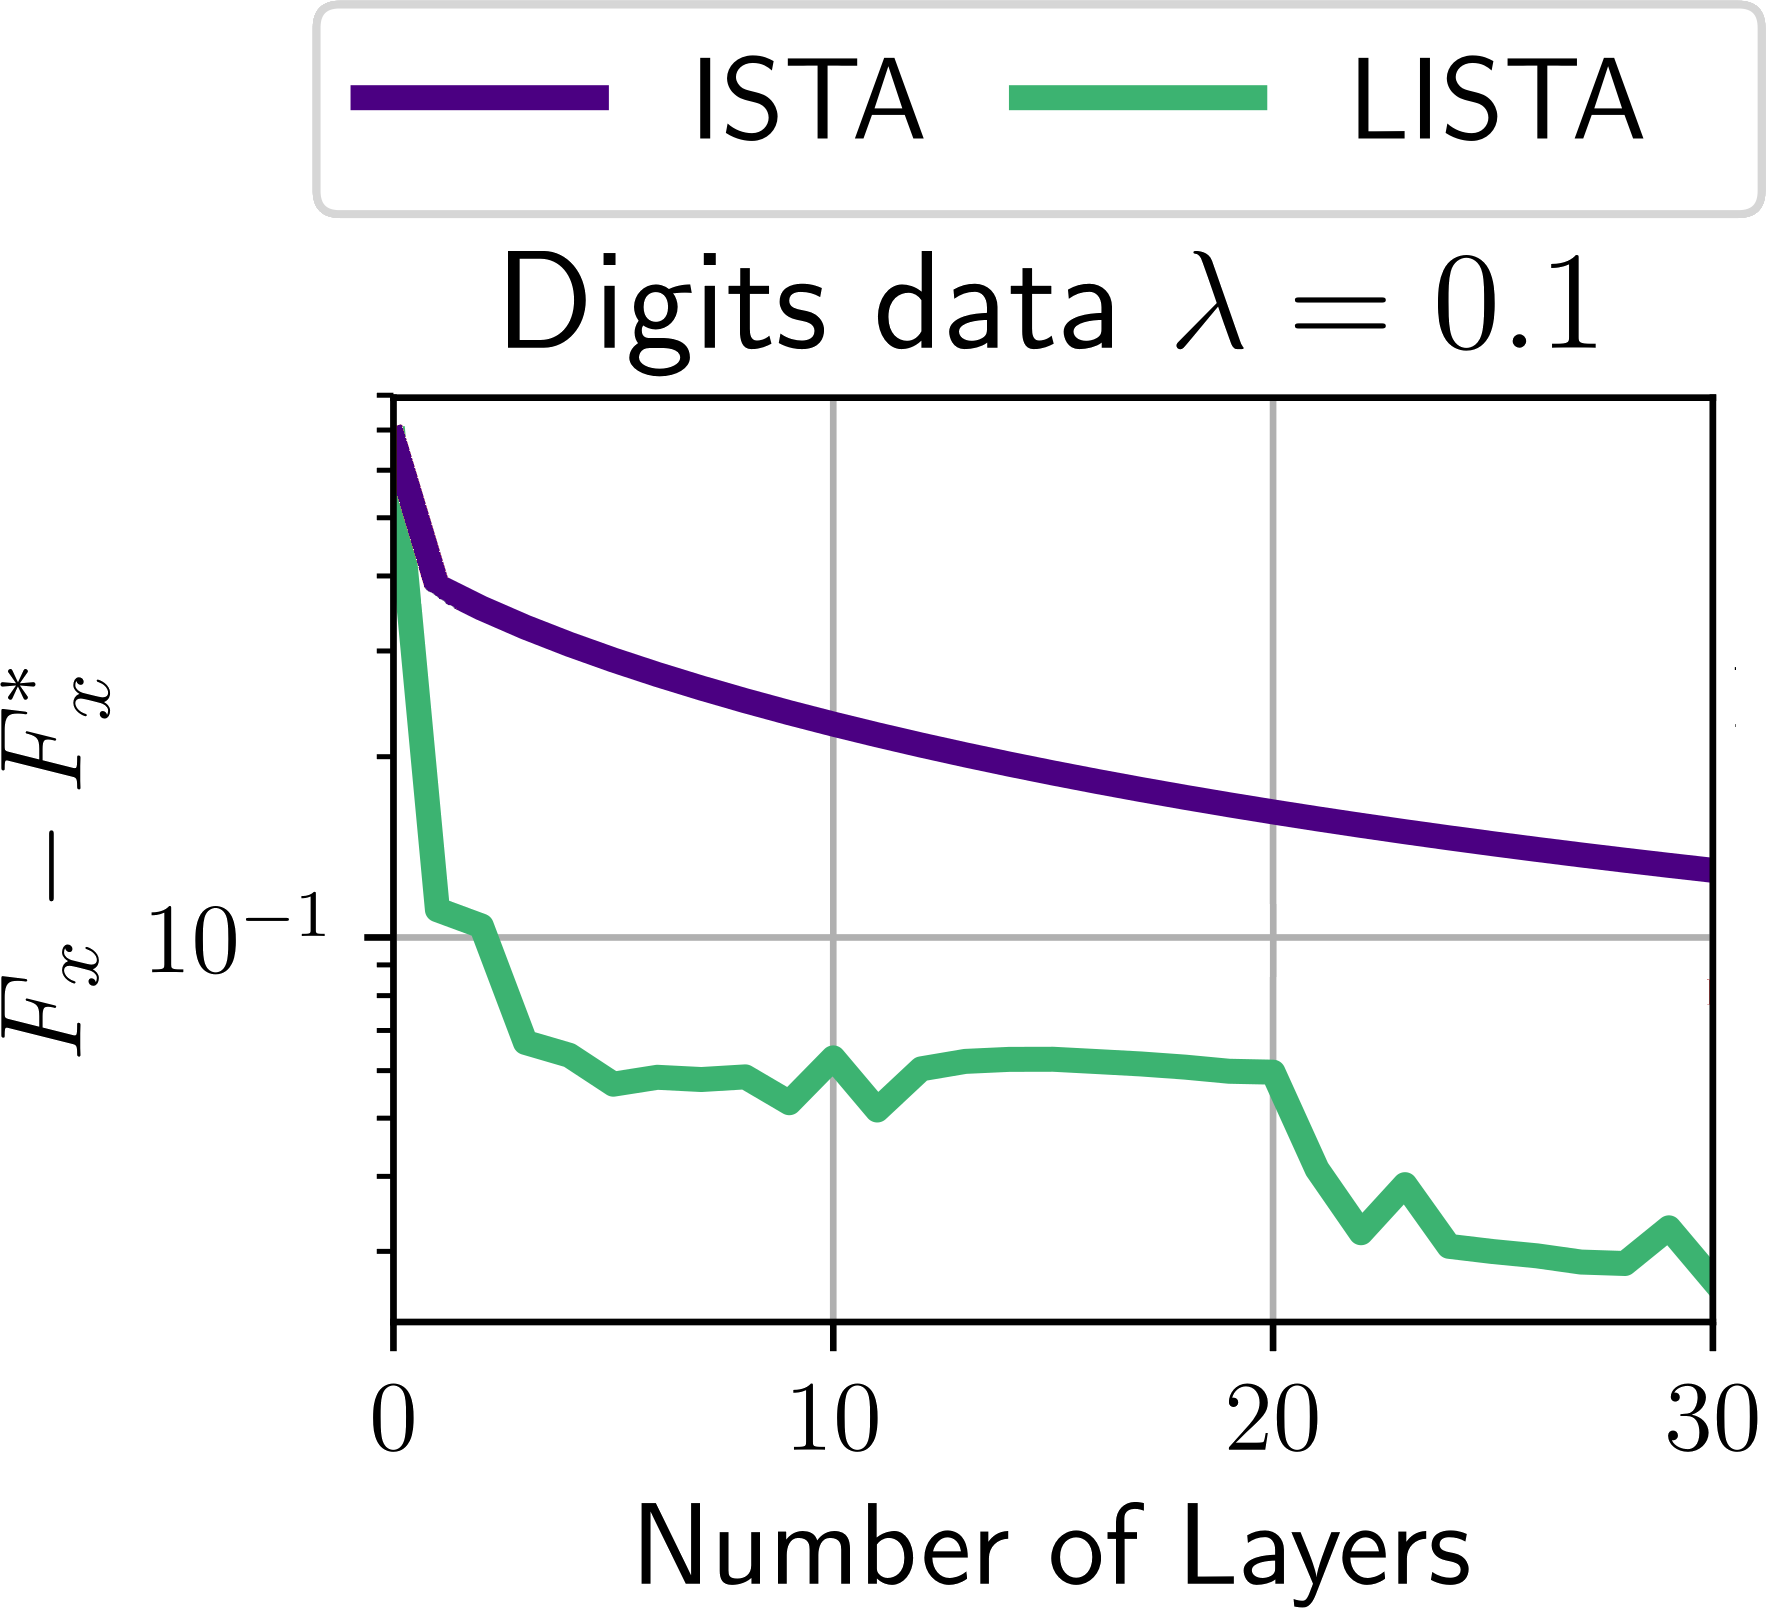
\includegraphics[width=.9\textwidth]{comparison_lista.png}\\}
        \end{columns}
    }

}

% 
\section{Learning to optimize with unrolled ISTA}
\parttitleframe{Moreau2017a,Ablin2019}


% \frame{
%     \frametitle{Solving many inverse problems}


%     \hskip-.7ex{\bf Context:} Many inverse problems with the same structure $G$.\\[1em]
%     \myitem{} One per time sample for MEG: $> 50k$ instances.\\[1em]
%     \begin{columns}[c]

%         \column{.55\textwidth}

%         {\bf Goal:} learn $\Phi_\Theta$ with $T$ layers such that:
%         \[
%             F_x(\Phi_\Theta(x)) \le F_x(ISTA_T(x))
%         \]
%         \strongpoint{Find the same solution as ISTA!}

%         \vskip1em

%         {\bf Questions:}\\[1em]
%         \myitem{} How fast can LISTA go?\\[.5em]
%         \myitem{} What does LISTA learn?\\[1em]

%         \column{.45\textwidth}
%         {\centering
%         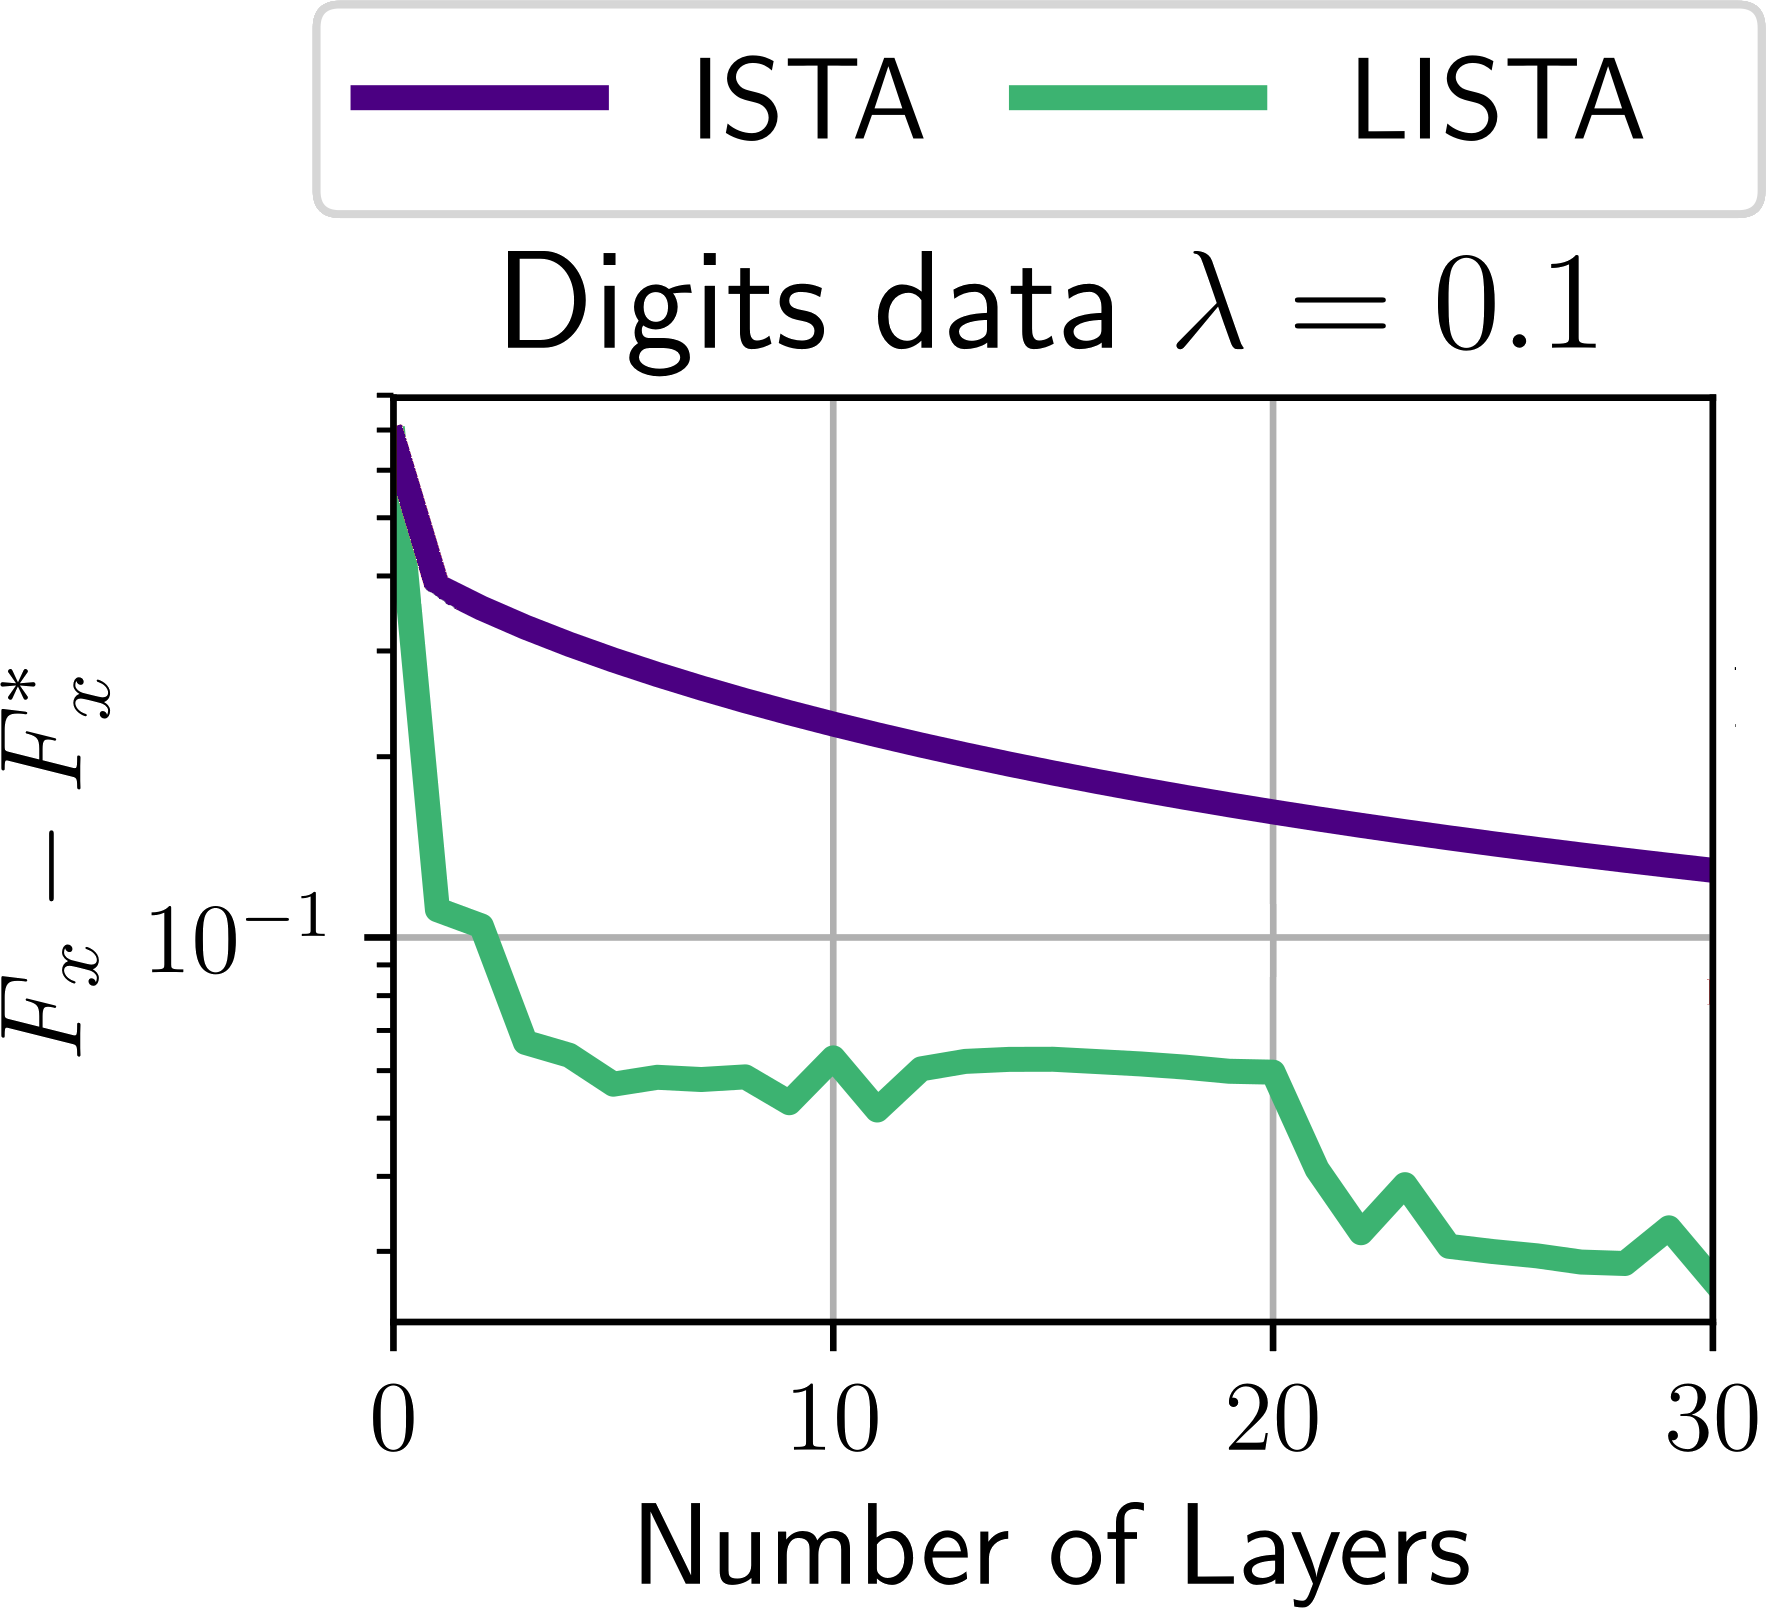
\includegraphics[width=\textwidth]{comparison_lista.png}\\}
%     \end{columns}
% }


\frame{
    \frametitle{How fast can LISTA go? \contrib{Moreau and Bruna, 2017}}

    Results are based on a quasi-diagonalization $G^\top G \simeq V^\top \Lambda V$ that does not distort ``too much'' the $\ell_1$-norm.\\[2em]

    \myitem{} For a class of parameters, LISTA has the same cvg rate as ISTA.\\[1em]
    \myitem{} LISTA can benefit from improved constants.\\[1em]
    \myitem{} As the optimization approaches a solution, it is harder and harder to get improved constants.\\[2em]


    \strongpoint{Shows that it is possible to improve the first iterations of the algorithm.}
}



\begin{frame}[t]{ISTA: Majoration-Minimization}
    Taylor expansion of $f_x$ in $z^{(t)}$
    \begin{align*}
        F_x(z) &  = f_x(z^{(t)}) + \nabla f_x(z^{(t)})^\top(z - z^{(t)})
                    + \frac{1}{2}\|G(z-z^{(t)})\|_2^2+ \lambda\|z\|_1\\
               & \le f_x(z^{(t)}) + \nabla f_x(z^{(t)})^\top(z - z^{(t)}) + \frac{L}{2}\|z - z^{(t)}\|_2^2 + \lambda\|z\|_1
    \end{align*}
    $\Rightarrow$ Replace the Hessian $G^\top G$ by an upper bound $L \textbf{ Id}$.\\[2em]

    \only<1>{
    Separable function that can be minimized in close form
    \begin{align*}
        \argmin_z \frac{L}{2}\left\|z^{(t)} - \frac{1}{L}\nabla f_x(z^{(t)}) - z\right\|_2^2 + \lambda\|z\|_1
        & = \text{prox}_{\frac{\lambda}{L}}\left(z^{(t)} - \frac{1}{L}\nabla f_x(z^{(t)})\right)\\
        & = \text{ST}\left(z^{(t)} - \frac{1}{L}\nabla f_x(z^{(t)}),
                           \frac{\lambda}{L}\right)
    \end{align*}
    }
    \only<2>{
        By design,
        \[
            F(z^{t+1}) \le Q^t(z^{t+1}) \le Q^t(z^{t+1}) = F(z^t)
        \]
        and the algorithm converges.\\[2em]
        The key is to find a majorant easy to minimize.
    }
\end{frame}


\begin{frame}{ISTA: Majoration for the data-fit}
    \definecolor{darkgreen}{RGB}{0, 148, 0}
    \myitem{} Level sets for $z^\top G^\top G z
                       \only<2>{\le \color{red} L \|z\|_2}
                       \only<3>{\le \color{blue} z^\top V^\top \Lambda V z}$
              \only<3>{\contrib{Moreau and Bruna, 2017}}\\
    \centering
    \makebox[.75\textwidth][c]{
        \only<1>{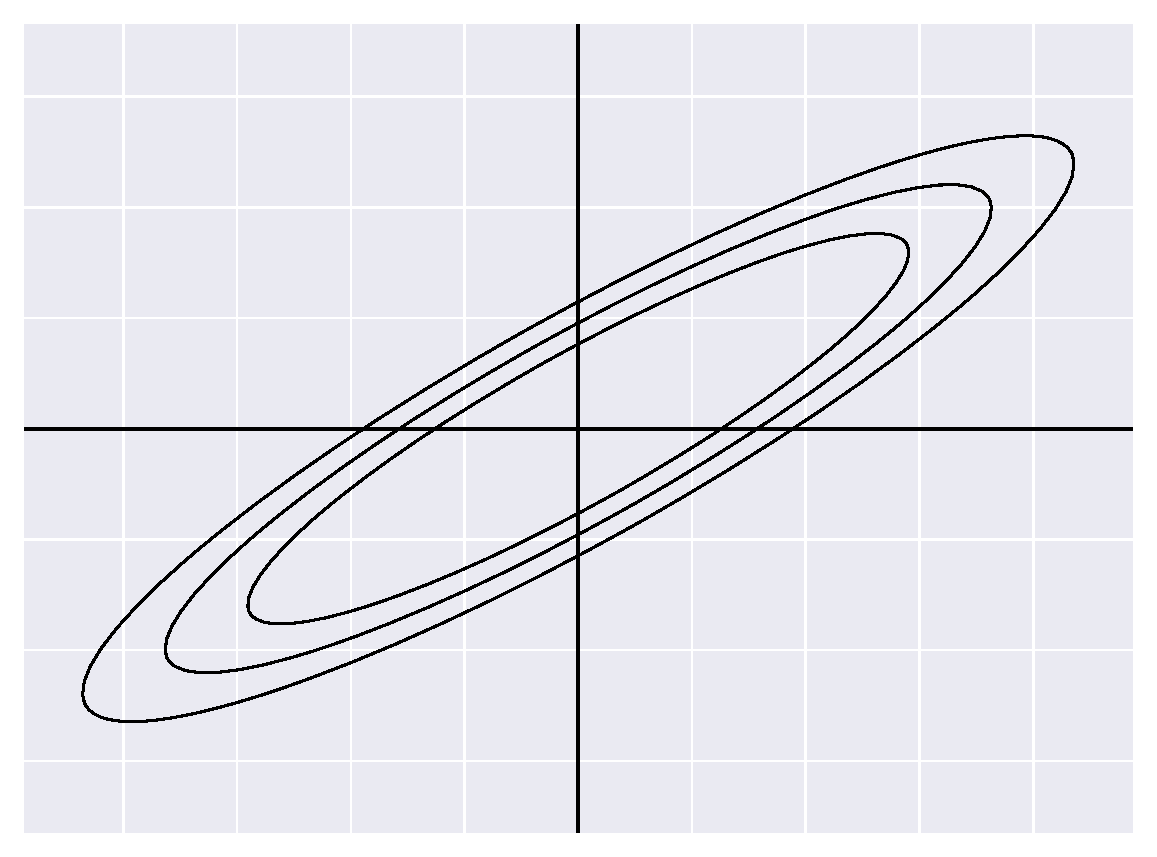
\includegraphics[height=.75\textheight]{ell1}}%
        \only<2>{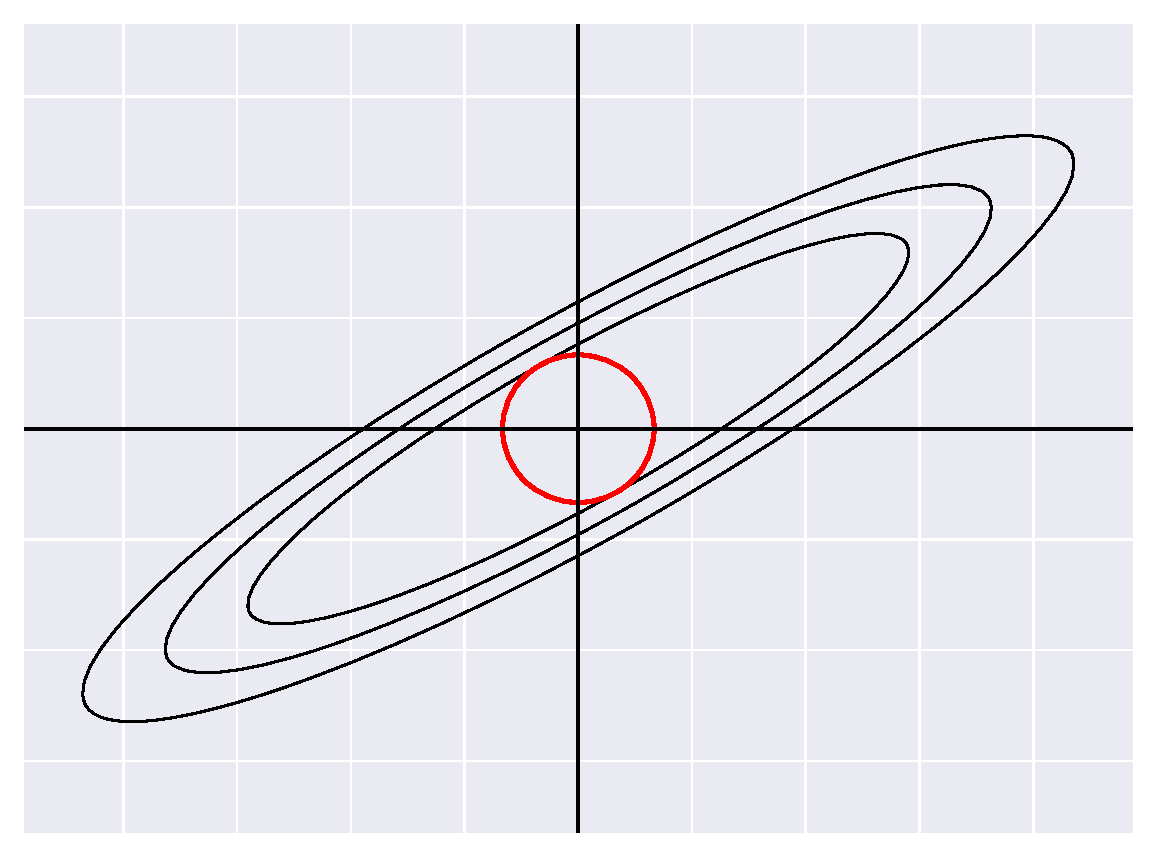
\includegraphics[height=.75\textheight]{ell2}}%
        \only<3>{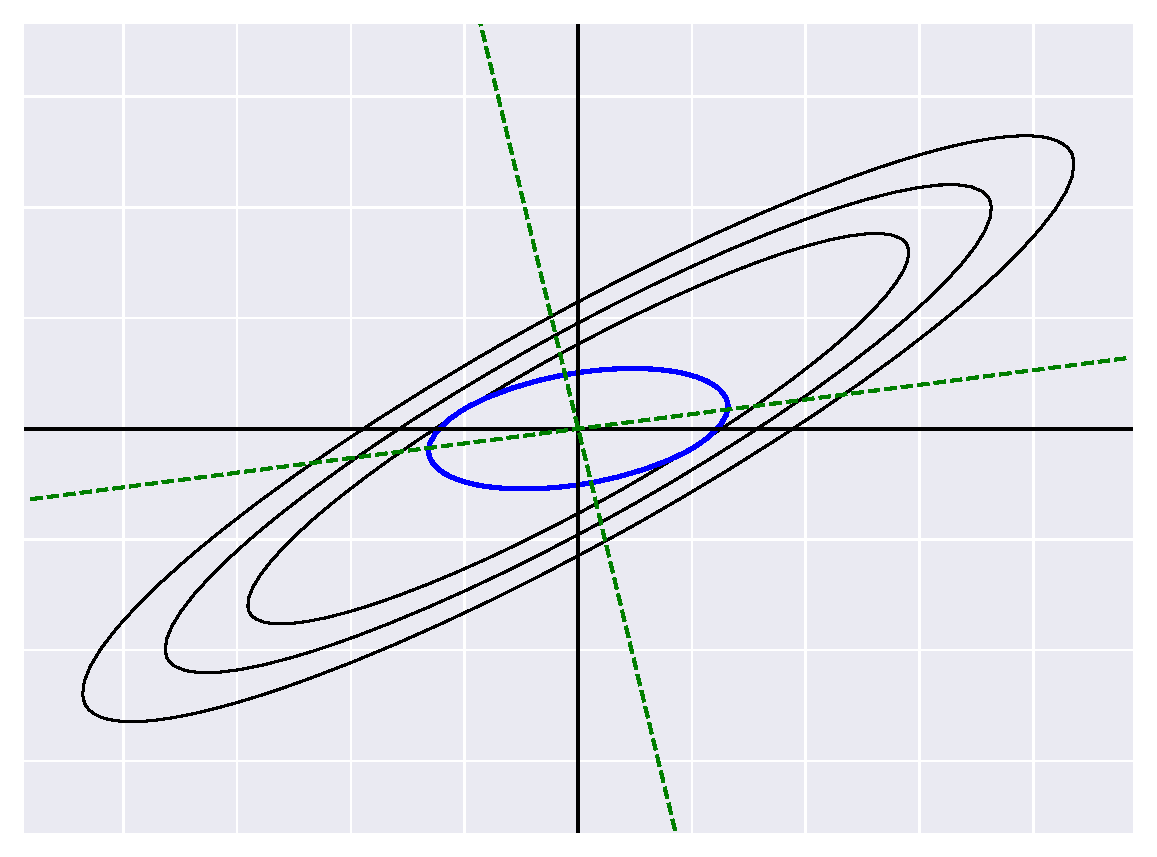
\includegraphics[height=.75\textheight]{ell3}}
    }\\
\end{frame}


\frame{
    \frametitle{What does LISTA learn? \contrib{Ablin et al., 2019}}

    Consider that the number of layers goes to $+\infty$.\\[1em]
    \begin{block}{Theorem -- Asymptotic convergence of the weights}
        Assume that the weights of the network converge to a limit:
        \[
            W_z^{(t)}, W_X^{(t)}, \beta^{(t)} \to W_z^*, W_X^*, \beta^*
            \qquad as \qquad t\to +\infty
        \]
        and that the output of the network converges to a solution of the unsupervised problem.\\[.5em]
        Then
        \[
            W_z^* = Id - \alpha D^\top D, \quad
            W_X^* = \alpha D^\top, \quad
            \beta^* = \alpha \lambda, \quad
        \]
    \end{block}

    \strongpoint{Correspond to ISTA with a learned step size $\alpha$}
}

% \frame{
%     \frametitle{Intuition for the result}

%     The network's output $\Phi(x)$ for all input $x$ needs to verify:
%     \begin{align*}
%         \Phi(x) = & ~ st\big(
%             \textcolor{linkcolor}{(Id - \frac1L G^\top G)}\Phi(x)
%             + \textcolor{D}{\frac1L G^\top} x,
%             \textcolor{Z}{\frac\lambda{L}}
%         \big) \qquad\qquad\keypoint{\text{KKT}}\\[.5em]
%         \Phi(x) = &~st\big(
%             \textcolor{linkcolor}{W_z^*}\Phi(x)
%             + \textcolor{D}{W_X^*} x,
%             \textcolor{Z}{\beta^*}
%         \big) \qquad\qquad\quad\keypoint{\text{Weights cvg}}
%     \end{align*}
%     \vskip2em
%     \myitem{} If verified uniformly, this imposes a strong structure on the asymptotic weights.\\[1em]
%     \myitem{} This structure can be relaxed based on the distribution of $x$.
% }

\begin{frame}{Numerical verification}
    \centering
    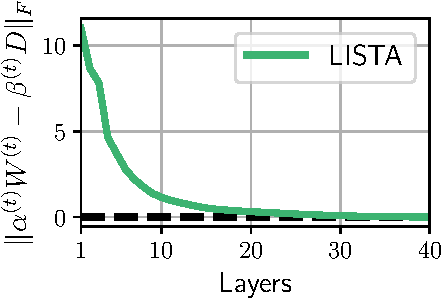
\includegraphics[width=.8\textwidth]{fro_similarity}\\[1em]
    40-layers LISTA network trained on a $10 \times 20$ problem with $\lambda = 0.1$\\
    {\bf The weights $W^{(t)}$ align with $D$ and $\alpha, \beta$ get coupled.}


\end{frame}


\begin{frame}{Step LISTA \contrib{Ablin et al., 2019}}

    Inspired by this result: learn adapted step sizes for ISTA.\\[2em]
    {\bf Restricted parametrization :}
    Only learn a step-size $\alpha^{(t)}$\\[1em]
    \[
    z^{(t+1)} = \text{ST}\left(z^{(t)}
              - \textcolor{linkcolor}{\bf\alpha^{(t)}} D^\top(D z^{(t)} -x),
              \lambda\textcolor{linkcolor}{\bf\alpha^{(t)}}\right)
    \]
    \vskip1em
    \underline{Fewer parameters:}\\[1em]
    % $T$ instead of $( 2 + mn)T~.$\\[1em]
    \begin{columns}[c]
        \column{.5\textwidth}
            \myitem{} Easier to learn\\
        \column{.5\textwidth}
            \myitem{} Fewer degrees of freedom\\
    \end{columns}
    \vskip2em
    \centering $\Rightarrow$ Reduced performances?\\

\end{frame}




\begin{frame}[t]{Performances}

    {\bf Simulated data:} $m=256$ and $n=64$\\[.7em]
    \hskip6ex $D_k \sim \mathcal U(\mathcal S^{n-1})$ and $x = \frac{\widetilde x}{\|D^\top \widetilde x\|_\infty}$ with $\widetilde x_i \sim \mathcal N(0, 1)$\\[1.5em]
    {\centering
    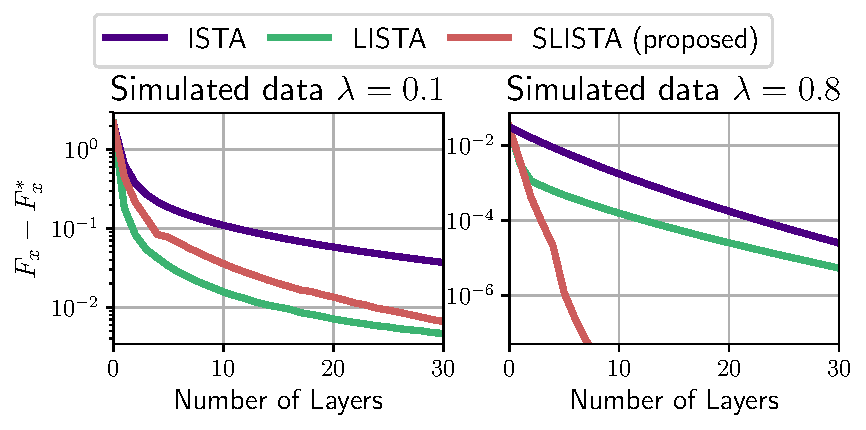
\includegraphics[width=\textwidth]{comparison_networks_simu}\\}
\end{frame}


\begin{frame}{Learning better step sizes}
    Linked to SLISTA when step sizes are in $\big[\frac1{L_S}, \frac2{L_S}\big[$ when $Supp(z^{(t)}) = S$\\[.5em]
    $L_S$ is the largest eigenvalue of $G^\top G$ restricted on the support $S$\[
        \max_{\substack{Supp(z) = S\\\|z\|_2\le 1}} z G^\top G z
    \]
    \centering
    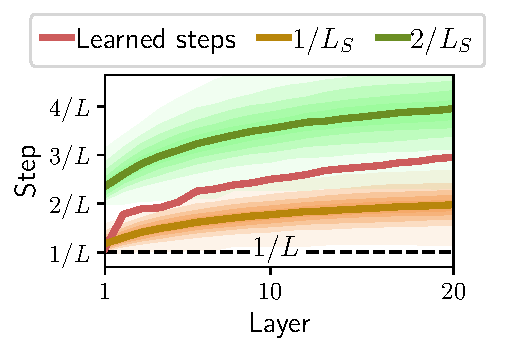
\includegraphics[width=.6\textwidth]{learned_steps}\\
    % The learned step-sizes are linked to the distribution of $1/L_S$\\[1em]


\end{frame}


\frame{
    \frametitle{Unrolling for learned optimization}

    \vskip4em
    {\centering\bf No hope to learn an algorithm that converges\\faster than ISTA \underline{uniformly}.\\[2em]}

    \begin{itemize}\itemsep.5em
        \item But one can learn parameters (step-size) of the algorithm that better adapt to the input distribution.\\
        \contrib{Ablin et al., 2019}
        \item Also possible to improve the first iterations of ISTA (improve constants).\\
        \contrib{Moreau and Bruna, 2017}
    \end{itemize}

    \vspace{0pt plus 1 filll}
    \footnotesize
    Also considered unrolled algorithms for TV in  Cherkaoui, Sulam, {\bf M.}, NeurIPS 2020.

}


\end{comment}

\section{A bilevel view on prior learning with unrolling}
\parttitleframe{Ablin2020,Malezieux2022a}

% \section{Learning $\mathcal R$ with unrolled algorithm}
% \parttitleframe{Malezieux2022a}


\frame[t]{
    \frametitle{Unrolling with min-min problems}

    \setbeamercovered{invisible}

    {\bf Bi-level formulation:}
    \[
        \min_{\theta\in \mathcal C} h(\theta) \triangleq F(\theta, \varZ^*(\theta))
        \quad s.t. \quad
        \varZ^*(\theta) = \argmin_z F(\theta, z)
        \enspace.
    \]
    Optimization problem in $D$ solved with projected gradient descent.\\
    \strongpoint{
        How to estimate the gradient $g^*(\theta) = \nabla h(\theta)$ efficiently?
    }\vskip1em

    \only<2-3>{

        {\bf Danskin Theorem:} \mycite{Danskin1967}
        \[
           g^*(\theta) = \nabla_1 F(\theta, \varZ^*(\theta))
        \]
        \emph{This is due to the fact that ``~$\nabla_2 F(\theta, \varZ^*(\theta)) = 0$''.}\\[2em]

        \visible<3>{{\bf Issue:} computing $\varZ^*(\theta)$ is computationally expansive.}
    }
}

\frame[t]{
    \frametitle{Unrolling with min-min problems}
        \textbf{Unrolled formulation:}\\[.5em]
    \[
        \min_{\theta\in\mathcal C} h_N(\theta) \triangleq F(\theta, \varZ^N(\theta))
        \enspace.
    \]
    The gradient estimate becomes:
    \[
        g^2_N(\theta) = \nabla_1 F(\theta, \varZ^N(\theta)) + J_N^\top\nabla_2 F(\theta, \varZ^N(\theta))
    \]
    Estimate the jacobian $J_N = \frac{d \varZ^N}{d \theta}$ with back-propagation.
    % \vskip1em
    % \begin{columns}
    %     \column{.39\textwidth}
    %         \underline{Re-parametrization:}\\[.5em]
    %         \myitem{} $W_X = \frac{D^\top G^\top}{L} $\\
    %         \myitem{} $W_z = Id - \frac{D^\top G^\top GD}{L}$
    %     \column{.59\textwidth}
    %         {\centering\inputTikZ{.5}{ista_unrolled}\\[1em]}
    % \end{columns}
    \only<2>{
        \vskip1em
        {\centering
        \highlight{
            {\bf Question:} More efficient to use unrolling than classic AM?
        }\\}

        \vskip2em
        \myitem{} Work for smooth problems.\contrib{Ablin et al., ICML 2020}\\[1em]
        \myitem{} Improved performances for supervised learning.\mycite{Monga2021}\\
    }


}


% \frame[t]{
%     \frametitle{What is optimized with unrolling?}

%     Consider the optimization problem:
%     \[
%         z^*(\varX; \theta) = \argmin_z G(z, \varX; \theta)
%     \]
%     If $\Phi_\Theta$, with $\Theta = (\theta, \lambda)$ corresponds to the unrolling of an algorithm computing $z*$, then learning $\Theta$ amounts to solving:
%     \begin{align*}
%         \min_\theta {\coloron{2}{darkblue}h(\theta)} = \underbrace{\mathbb E_{\varZ, \varX}[\|\varZ - z^*(\varX; \theta)\|_2^2]}_{\coloron{2}{darkred} F(z^*(\varX; \theta))}\\
%         \text{s.t.}\quad z^*(\varX; \theta) = \argmin_z {\coloron{2}{lightgreen} G(z, \varX; \theta)}
%     \end{align*}
%     \only<2>{
%     \begin{tikzpicture}[overlay]
%         \draw[<-, thick, shorten >=8, darkblue] (4.1, 1.8) -- +(-2.3, -1.3) node[darkblue] {\emph{Value function}};
%         \draw[<-, thick, shorten >=35,darkred] (7.8, 1.5) -- +(3, -.2) node {\emph{\color{darkred}Outer function}};
%         \draw[<-, thick, shorten >=8, lightgreen] (8, .5) -- +(0, -.8) node {\emph{\color{lightgreen} Inner function/Problem}};
%     \end{tikzpicture}
%     }
%     \only<3->{
%         Can compute its gradient:
%         \[
%             \nabla h(\theta) = \nabla_\theta F({\coloron{4}{red}z^*}) + {\coloron{4}{red}\frac{\partial z^*}{\partial\theta}}^T\nabla_z F({\coloron{4}{red}z^*})
%         \]
%         \strongpoint{Need to compute $z^*$ and its jacobian.}
%     }
% }


% \frame[t]{
%     \frametitle{What is optimized with unrolling?}

%     With unrolling, we replace $z^*$ by $z^N$:
%     \begin{align*}
%         \min_\theta {h(\theta)} = \underbrace{\mathbb E_{\varZ, \varX}[\|\varZ - z^N(\varX; \theta)\|_2^2]}_{ F(z^N(\varX; \theta))}\\
%         \text{s.t.}\quad z^N \approx \argmin_z { G(z, \varX; \theta)}
%     \end{align*}
%     This simplifies computing the gradient:
%     \[
%         \nabla h(\theta) = \nabla_\theta F(z^N) + \underbrace{\frac{\partial z^N}{\partial\theta}^T\nabla_z F(z^N)}_{\text{Backpropagation}}
%     \]

%     \uncover<2>{\strongpoint{\bf
%         Does this converge to the same solution as the original problem?
%     }}

% }



\frame[t]{
    \frametitle{Gradient Estimation}

    \begin{columns}[T]
        \column{.45\textwidth}
        {\bf Alternate Minimization}\\[.5em]
        No Jacobian estimation
        \[
            g^1_N(\theta) = \nabla_1 F(\theta, \varZ^N(\theta))
        \]
        \column{.02\textwidth}
            \rule{.1mm}{.33\textheight}
        \column{.48\textwidth}
        {\bf Unrolling}\\[.5em]
        Account for Jacobian of $\varZ^N$
        \[
            \begin{split}
                g^2_N(\theta) = & \nabla_1 F(\theta, \varZ^N(\theta))\\
                   & + J_N^\top\nabla_2 F(\theta, \varZ^N(\theta))
            \end{split}
        \]
    \end{columns}

    \vskip1.5em
        \begin{columns}[T]
            \column{.45\textwidth}
            \only<2->{
                Converges as fast as $\varZ^N$
                \[
                    \|g^1_N - g^*\|_2 \le L_1 \|\varZ^N - \varZ^*\|_2
                \]
            }
            \column{.02\textwidth}
                \vskip-4em\rule{.1mm}{.52\textheight}
            \column{.48\textwidth}

            \only<3->{
                May converge faster than $\varZ^N$
                \[
                    \begin{split}
                        \|g^2_N - g^*\| \le & L\|J_N-J^*\|_2\|\varZ^N - \varZ^*\|_2\\
                                            & + L_2\|\varZ^N - \varZ^*\|_2^2
                    \end{split}
                \]
                \strongpoint{Need to study $\|J_N - J^*\|_2$.}
            }
        \end{columns}
}



\frame{
    \frametitle{Differentiable unrolling of $\varZ^N$}

    {\bf Idea:} \parbox[t]{.9\textwidth}{
        Compute $J_N = \frac{\partial \varZ^N}{\partial \theta}(\theta) \approx \frac{\partial \varZ^*}{\partial \theta}(\theta)$
        using automatic differentiation\\
        through an iterative algorithm.}\\[2em]

        \visible<2->{
            For the gradient descent algorithm:
            \[
                \varZ^{N+1} = \varZ^N - \rho \frac{\partial F}{\partial z}(\theta, \varZ^N)
            \]
            The Jacobian reads,
            \[
                \frac{\partial \varZ^{N+1}}{\partial \theta}(\theta) = \Big(Id - \rho\frac{\partial^2 F}{\partial z^2}(\theta, \varZ^N) \Big)\frac{\partial \varZ^N}{\partial \theta}(\theta) - \rho\frac{\partial^2 F}{\partial z\partial \theta}(\theta, \varZ^N)
            \]
        }
        \visible<3->{
            \strongpoint{Under smoothness conditions, if $\varZ^N$ converges to $\varZ^*$,\\this converges toward $\frac{\partial \varZ^*}{\partial \theta}(\theta)$}
        }
}

\frame{
    \frametitle{Analysis for min-min problems \rightcite{Ablin et al. 2020}}

    We consider the $3$ gradient estimates:
    \begin{itemize}
        \item  $g_1^N = \nabla_\theta F (\theta, \varZ^N)$ \keypoint{Analysis}
        \item  $g_2^N = \nabla_\theta F (\theta, \varZ^N)
            + \frac{\partial \varZ^N}{\partial \theta}^\top \nabla_z F (\theta, \varZ^N)
        $\keypoint{Automatic}
        \item  $g_3^N = \nabla_\theta F (\theta, \varZ^N)
        - \frac{\partial^2 G}{\partial z\partial \theta}(\theta, \varZ^N)\frac{\partial^2G}{\partial z^2}^{-1}(\theta, \varZ^N) \nabla_z F (\theta, \varZ^N)
        $\keypoint{Implicit}
    \end{itemize}
    \vskip1em
    \visible<2->{
        \begin{columns}
        \column{.55\textwidth}
        {\bf Convergence rates:} For G strongly convex in $z$,
        \begin{align*}
            |g^N_1(x) - g^*(x)| &= O\left(|\varZ^N(\theta)  - \varZ^*(\theta) |\right), \\
            |g^N_t(x) - g^*(x) | &= o\:\left(|\varZ^N(\theta)  - \varZ^*(\theta) |\right), \\
            |g^N_3(x) - g^*(x) | &= O\left(|\varZ^N(\theta)  - \varZ^*(\theta) |^2\right)  .
        \end{align*}
        \column{.4\textwidth}
        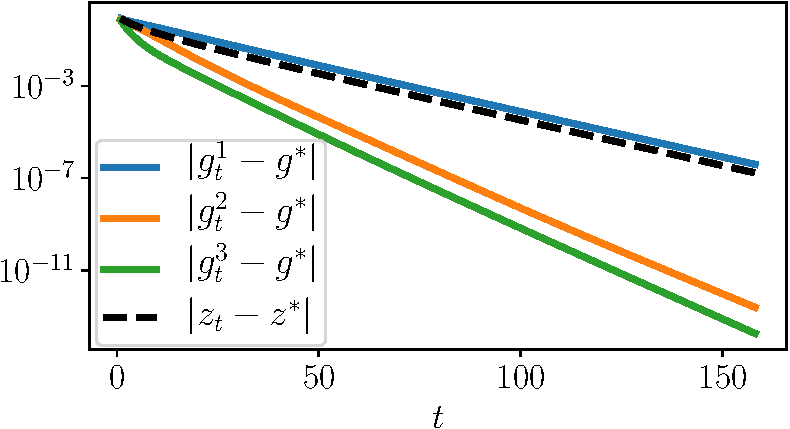
\includegraphics[width=\linewidth]{cvg_gradient}
        \end{columns}
    }

}

\frame{
    \Huge What about non-smooth problem?\\[2em]

    \normalsize
    Very common in inverse problem.\\[1em]
    \pause{}
    \strongpoint{Here, we consider the case of the Lasso.}

    \[
        \varZ^* = \argmin \|\varX - \varD D \varZ\|_2^2 + \lambda\|z\|_1
    \]
    with $\theta = D$.
}

\frame{
    \frametitle{Jacobian Estimation \contrib{Malézieux et al., 2022}}

    \begin{tcolorbox}[title=\textbf{Convergence of the Jacobian}]
        \[
        \|J_N - J^*\|_2 \le A_N + B_N \enspace .
        \]
        $A_N$ converges linearly towards 0, $B_N$ is an error term which may increase for large $N$ and vanishes on the support of $\varZ^*$.
    \end{tcolorbox}

    \vskip2em
    \myitem{} On the support, the jacobian converges linearly.\\[1em]
    \myitem{} Before reaching the support, $B_N$ is an error term that can accumulate.\\[1em]
    \myitem{} \parbox[t]{.8\textwidth}{
        $B_N$ can be attenuated with truncated back-propagation.
    }
}

\frame{
    \frametitle{Empirical evaluation}

    {\centering
    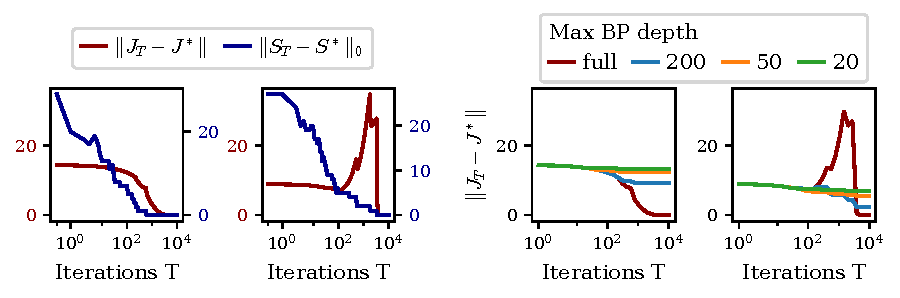
\includegraphics[width=.7\linewidth,trim={0 0 20em 0}, clip]{conv_jac.pdf}\\[1em]}

    \myitem{} Linear convergence once the support $S^*$ is reached.\\[1em]
    \myitem{} Possible explosion before reaching $S^*$.

}

\frame{
    \frametitle{Empirical evaluation}

    {\centering
    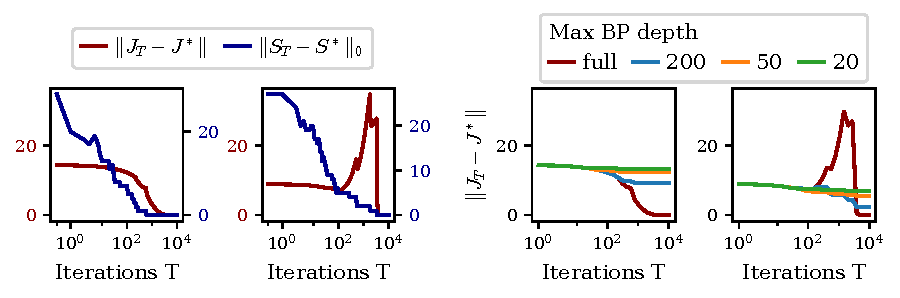
\includegraphics[width=.7\linewidth,trim={20em 0 0 0}, clip]{conv_jac.pdf}\\[1em]}

    \myitem{} Truncated backpropagation (BP) reduces the explosion.\\[1em]
    \myitem{} Less precise when the support is reached.

}



\frame{
    \frametitle{Numerical experiments on gradient}

    {\centering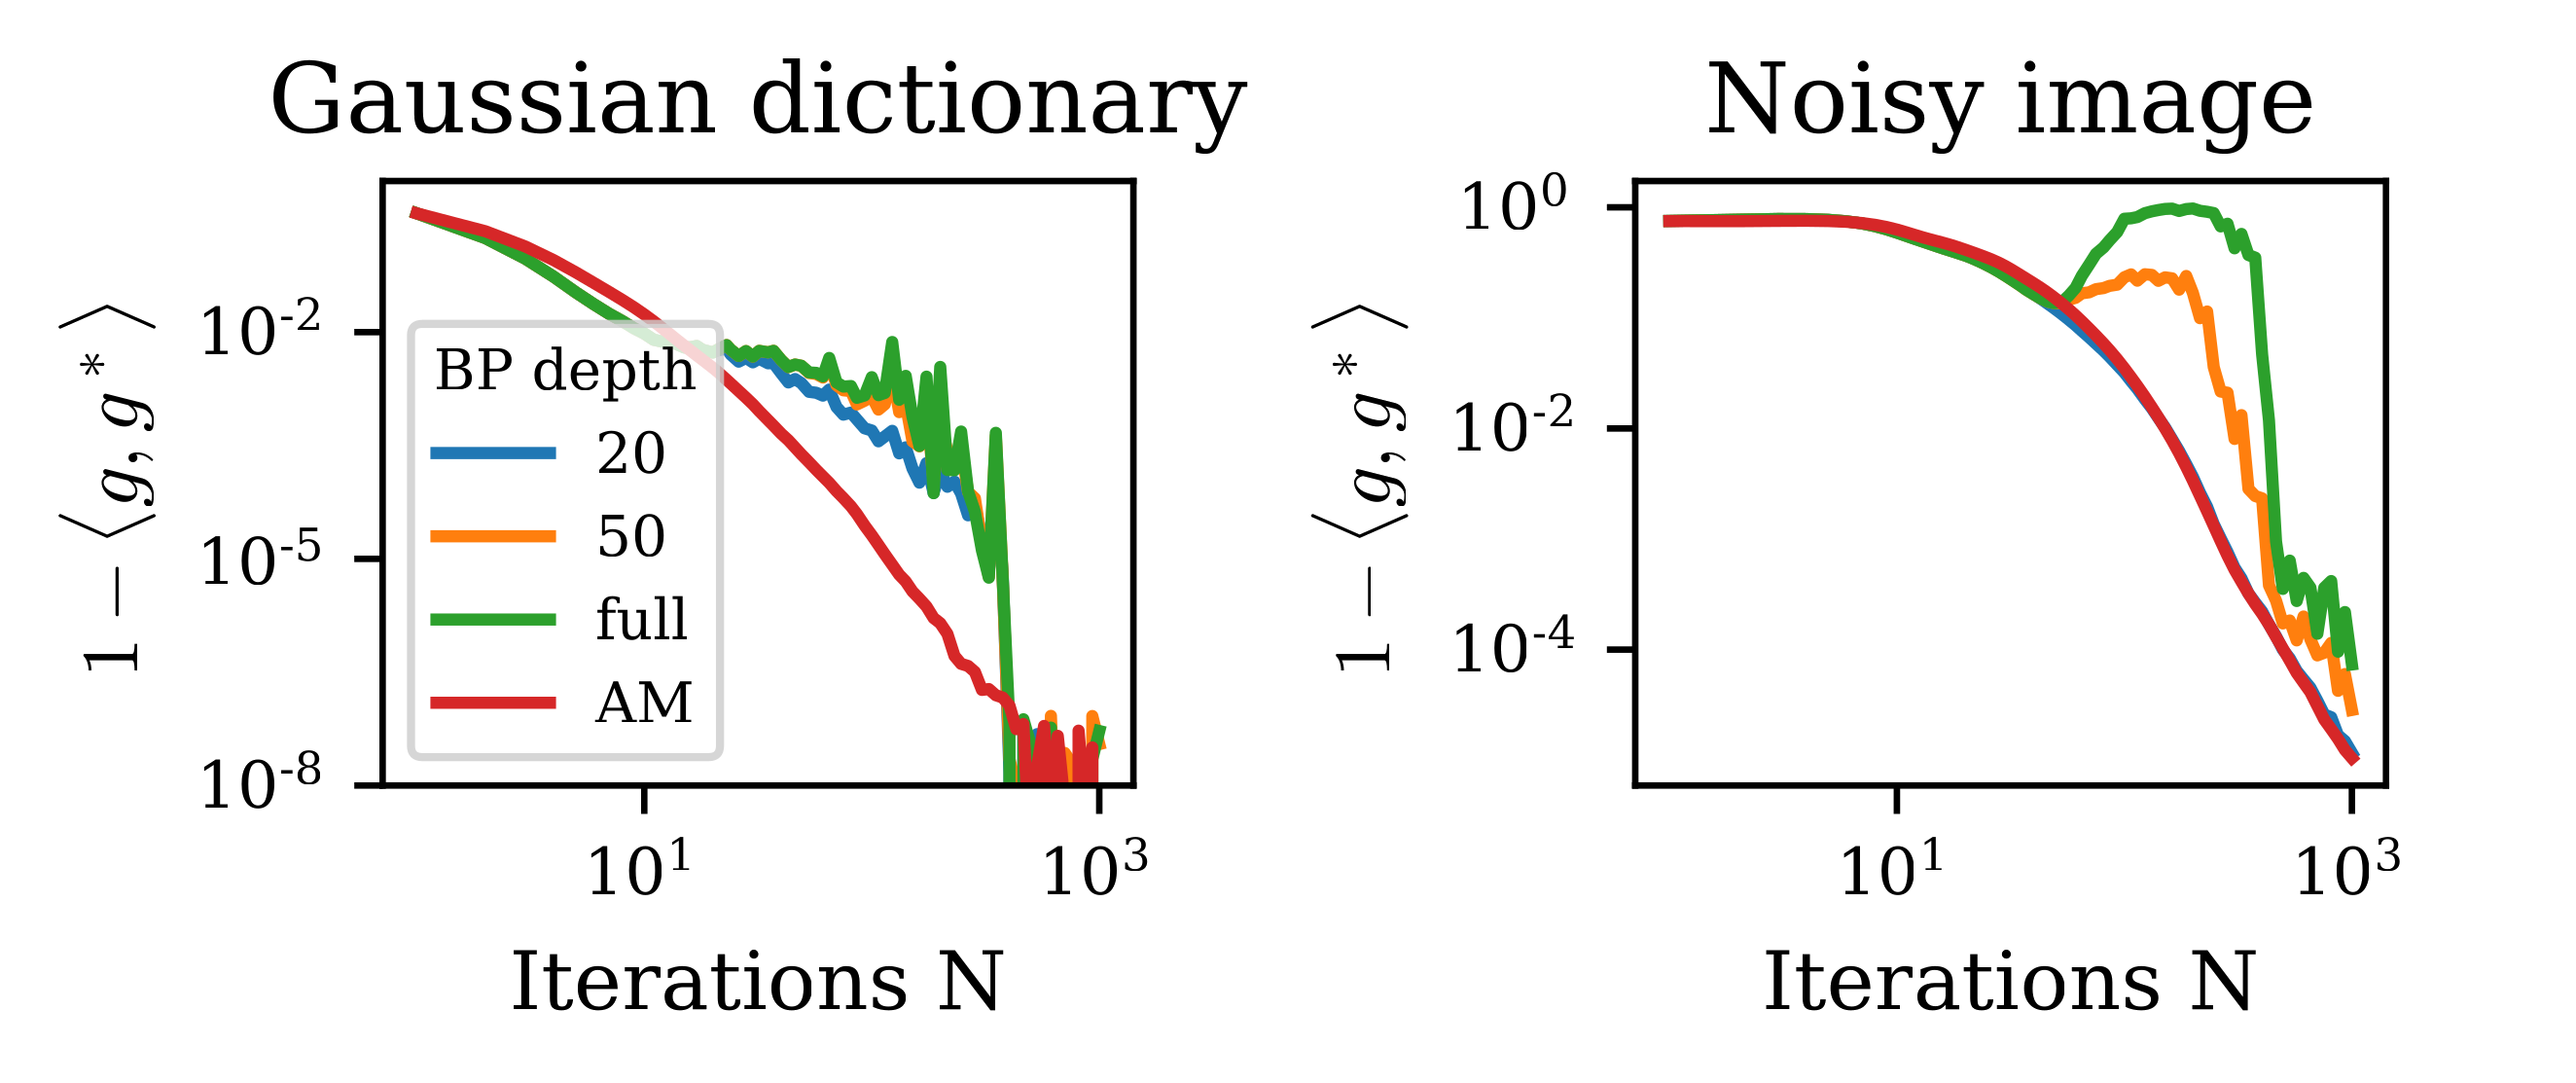
\includegraphics[width=.8\linewidth]{gradients_small.png}\\[1em]}
    \myitem{}\textbf{First iterations:} Stable behavior.\\[1em]
    \myitem{}\textbf{Too many iterations:}
        Numerical instabilities due to the accumulation of errors.
        Truncated back-propagation reduces the errors.\\[1em]
    \myitem{}\textbf{On the support:} Convergence towards $g^*$.
    \vskip1em
}


\frame{
    \frametitle{Unrolling for Jacobian estimation}

    {\centering\bf Not the expected performance boost in the non-smooth case.\\[1em]}

    \begin{itemize}\itemsep1em
        \item Jacobian estimate stable only for a very low number of iteration.
    \end{itemize}

    \strongpoint{
        What does this mean for unrolling?
    }

    \vskip2em
    \begin{itemize}\itemsep1em
        \item
        Still interesting to solve the problem:\\[.5em]
        \[
            \min_\theta \mathcal L(\varZ^N(\varX; \theta, \psi))
        \]
        with $\varZ^N(\varX; \theta, \psi)$ an unrolled algorithm with $N$ steps.
        \item But we are not optimizing for $\varZ^*$.
        \strongpoint{We are not independent of how we obtain $\varZ^N$.}
    \end{itemize}

}


\section{Iteration overfitting with unrolled optimization}
\parttitleframe{Ramzi2023}


\frame{
    \frametitle{Deqs -- Deep Equilibrium Networks}

    Consider the DEqs framework \emph{(more general than bilevel)}\\[.5em]
    \[
        \min_\theta \mathcal L(\varZ^*(\theta))
        \quad s.t. \quad
        \varZ^*(\theta) = f_\theta(\varZ^*(\theta))
    \]
    \vskip1em\pause{}
    In practice, solved as
    \[
        \theta^{*, N} = \argmin_\theta \mathcal L(\varZ^N(\theta))
    \]
    with $\varZ^N(\theta)$ obtained through $N$ iterations of an algorithm.\\[.5em]

    \emph{The promice of these models:} you can use $M > N$ during test time to get performance boost.
    \pause{}

    \strongpoint{
        Is this really true?
    }

}

\frame{
    \frametitle{Test-time fixed point computation \contrib{Ramzi et al., 2023}}

    If we learn $\theta^{*, N}$ with a given $N$, what can you say about $\mathcal L(z^{N + \Delta N}(\theta^{\star, N}))$?

    \pause{}
    \vskip2em


    \begin{tcolorbox}[title=\textbf{Theorem~1 -- Iteration overfitting}]
        Under simplifying hypothesis (linear DEqs), if $f_\theta$ is overparametrized, we have for all $\Delta N$:
       \begin{equation}
           \label{ineq:main-ineq-overparam}
           \mathcal L(z^{N + \Delta N}(\theta^{\star, N})) \geq \mathcal L(z^N(\theta^{\star, N})),
       \end{equation}
    \end{tcolorbox}

    \vskip1em
    We also show that the closer to overparametrized $f_\theta$ is, the less we expect to see improvement with $N + \Delta N$.
}

\frame{
    \frametitle{What happens in practice?}

    \textbf{Context:} Overparametrized DEQs.\\[2em]
    \centering
    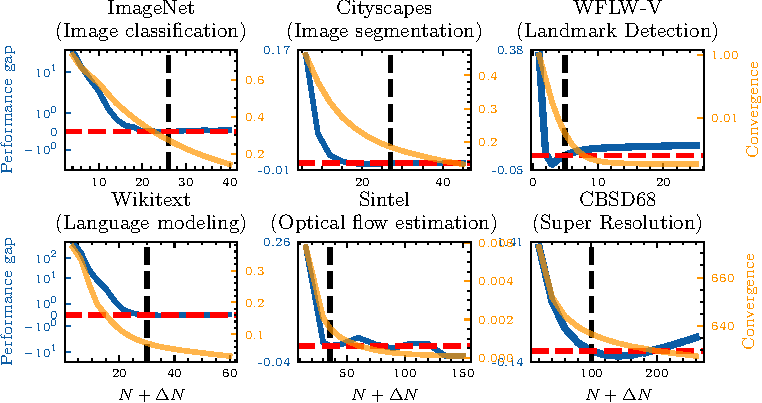
\includegraphics[width=\textwidth]{relative_error_vs_n_iters}\\
}

\frame{
    \frametitle{What happens in practice?}

    \textbf{Context:} Underparametrized Meta-learning.\\[2em]
    \centering
    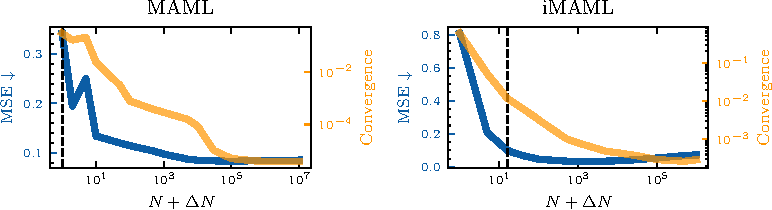
\includegraphics[width=\textwidth]{mse_vs_n_iters_maml}\\
}

\frame{
    \frametitle{Take-home message}


    \begin{itemize}\itemsep2em
        \item Unrolled networks work well for smooth minimization
        \item {\bf For non-smooth problems, the jacobian estimate is unstable}
        \item When training with fixed number of iterations, it makes sense to use the same number of iterations at test time.
    \end{itemize}
}



%%%%%%%%%%%%%%%%%%%%%%%%%%%%%%%%%%%%%%%%%%%%%%%%%%%%%%%%%%%%%%%%%%%%%%%%%%%%%%%
\begin{frame}[fragile]{Benchopt \rightcite{Moreau et al. 2022}}

Reproducing this comparison and adding solvers and tasks is easy as:\\[.5em]


\begin{center}
\begin{tabular}{c}
\begin{lstlisting}[language=bash,linewidth=.85\textwidth]
git clone https://github.com/benchopt/benchmark_bilevel
benchopt run ./benchmark_bilevel
\end{lstlisting}
\end{tabular}
\end{center}

\vskip.5em\centering
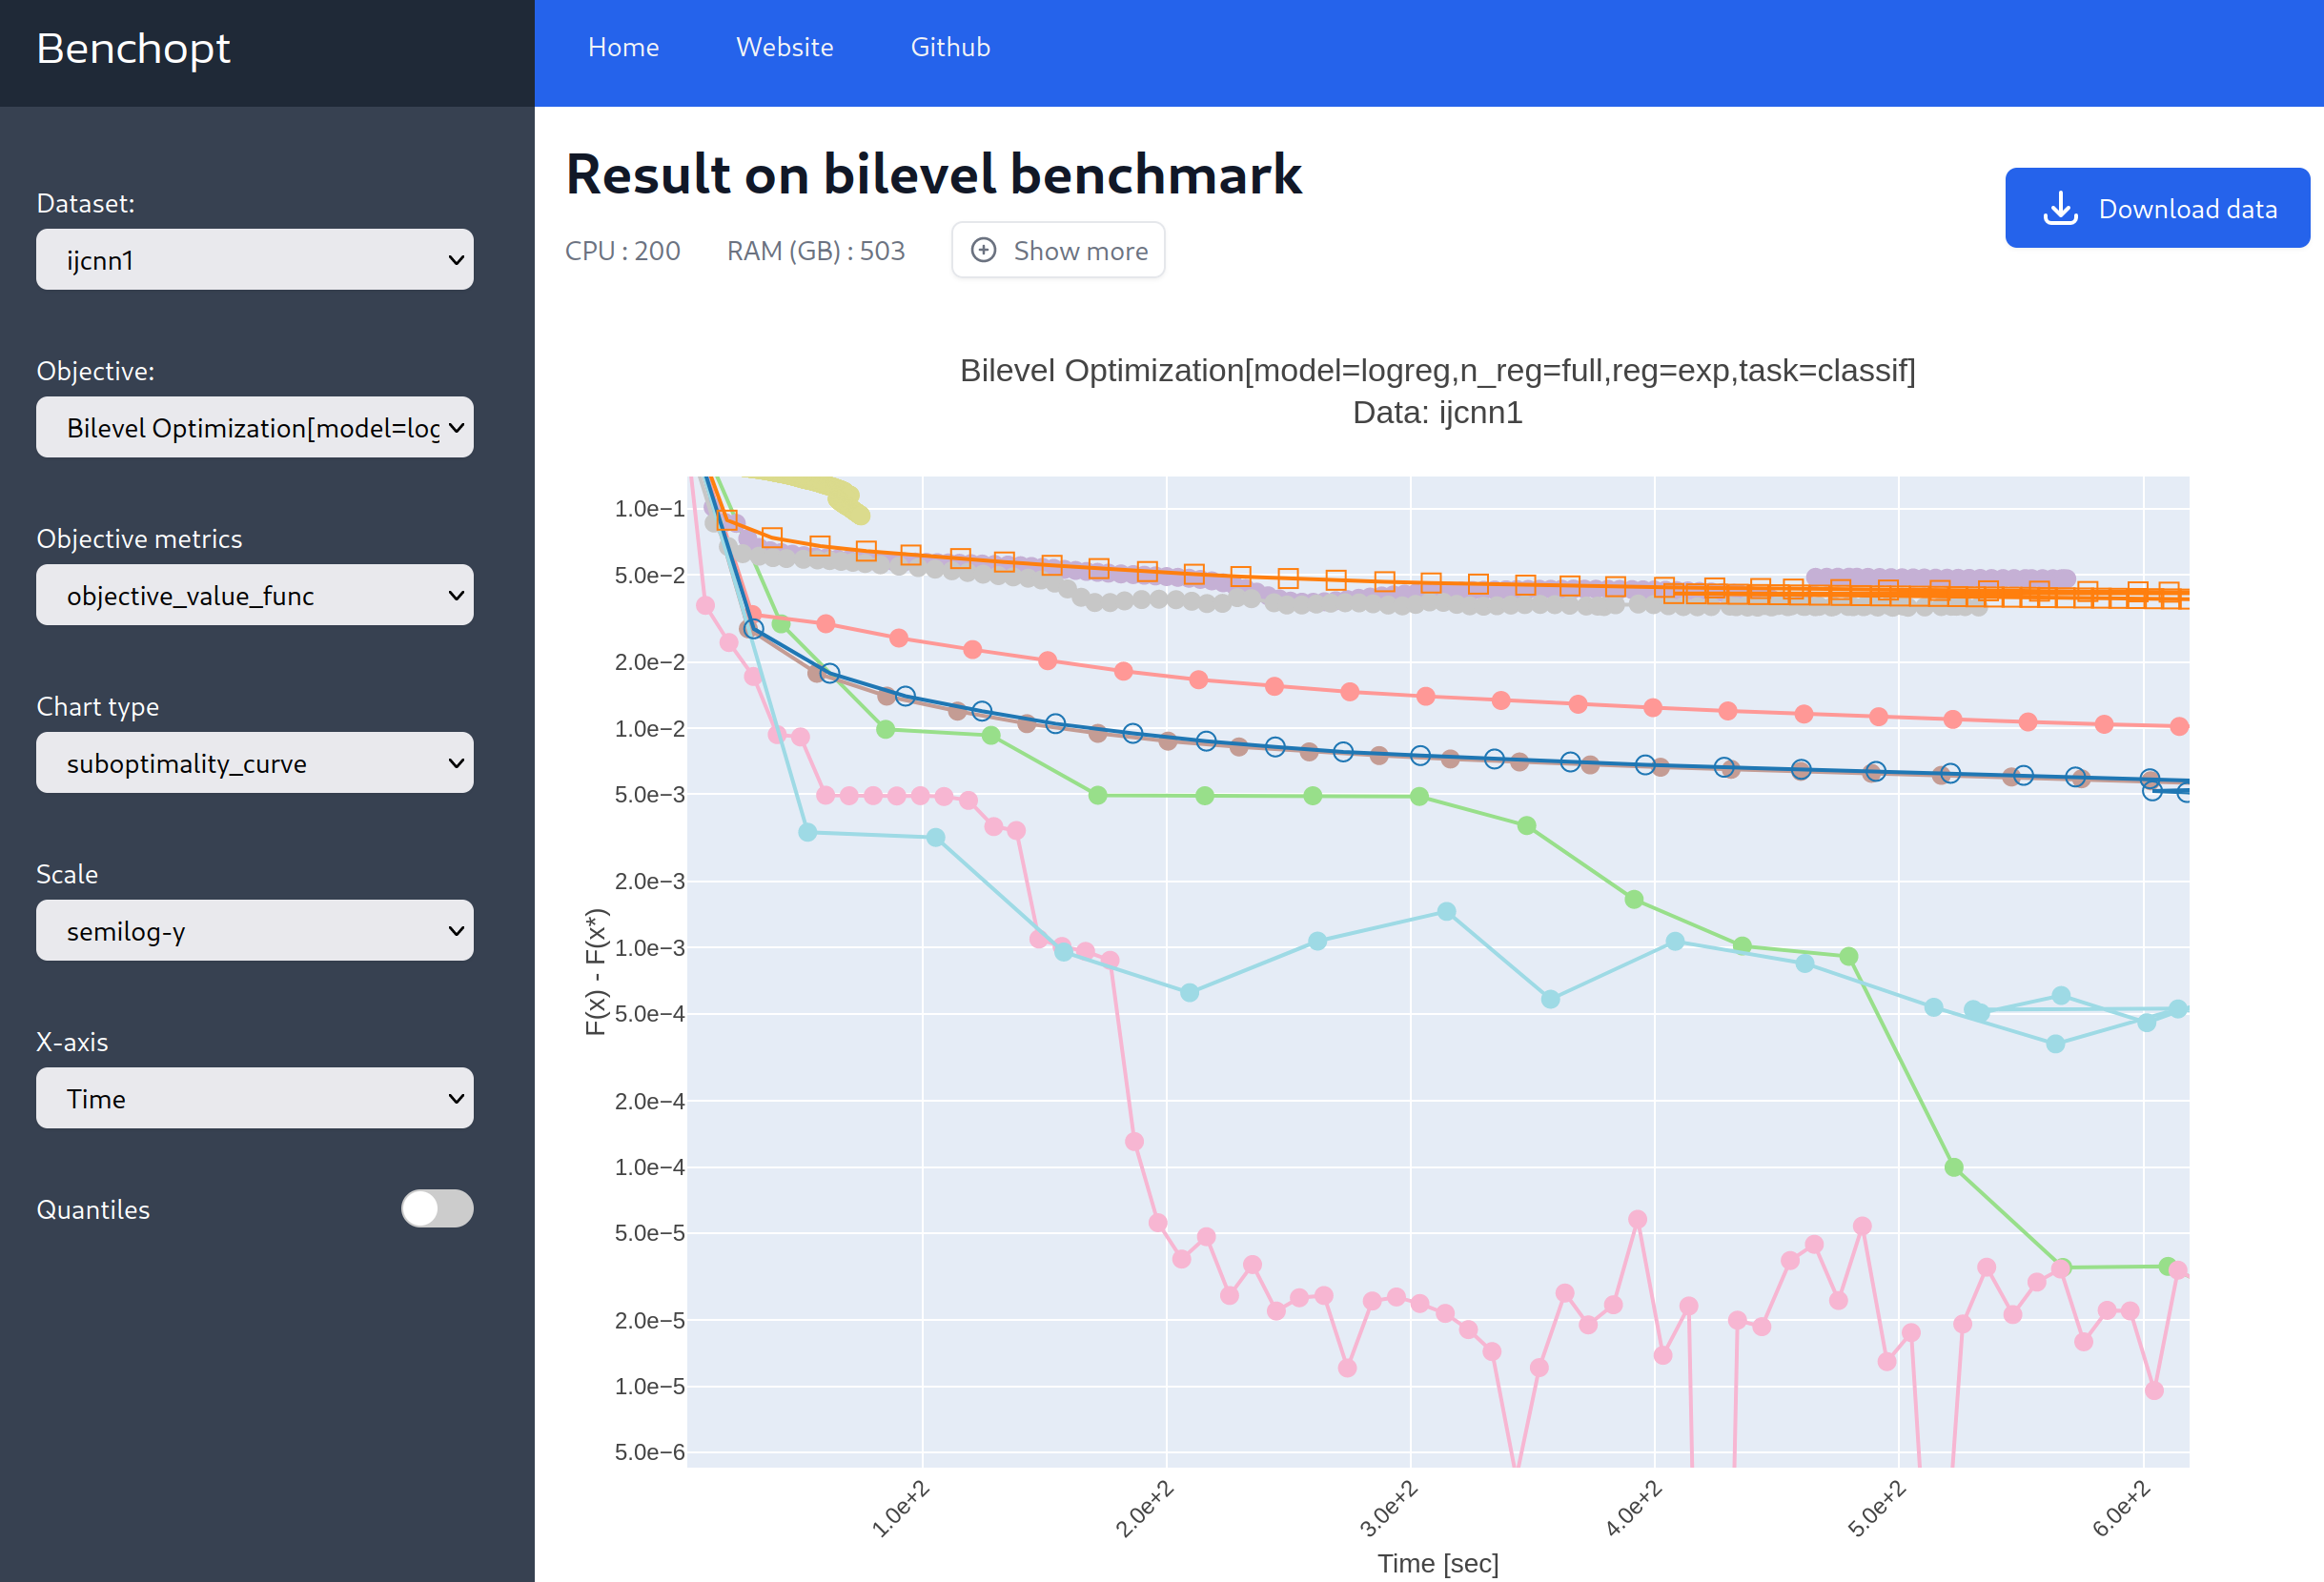
\includegraphics[width=.7\textwidth]{benchopt_bilevel}\\

% \hskip3ex
% 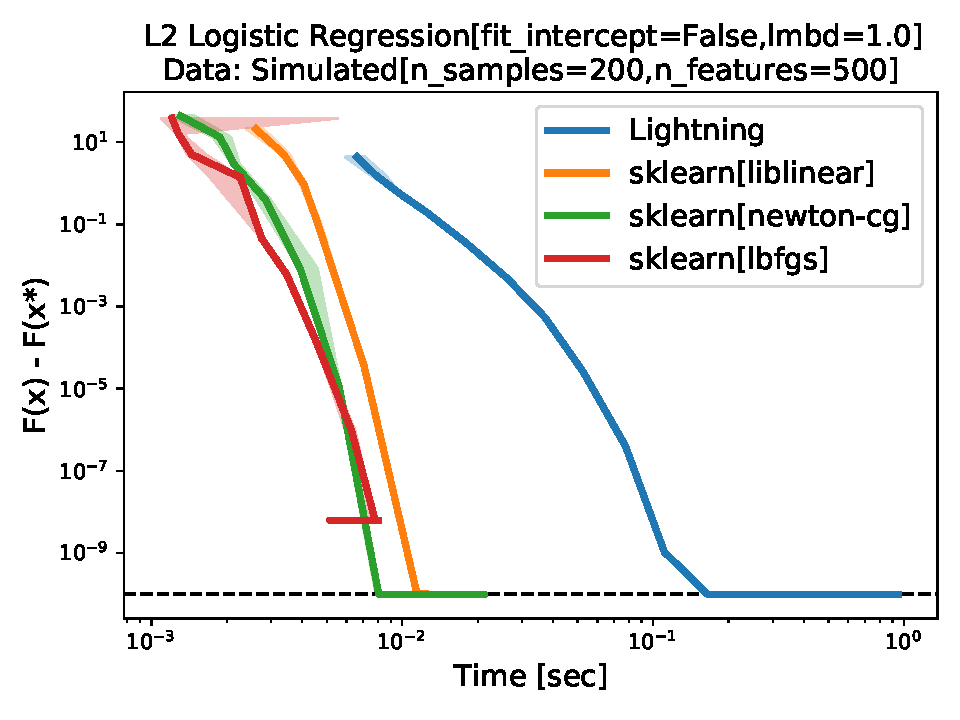
\includegraphics[width=.45\textwidth]{logreg_l2_1}

\end{frame}
%%%%%%%%%%%%%%%%%%%%%%%%%%%%%%%%%%%%%%%%%%%%%%%%%%%%%%%%%%%%%%%%%%%%%%%%%%%%%%%


%%%%%%%%%%%%%%%%%%%%%%%%%%%%%%%%%%%%%%%%%%%%%%%%%%%%%%%%%%%%%%%%%%%%%%%%%%%%%%%
\frame{
    \frametitle{Benchopt: principle}

    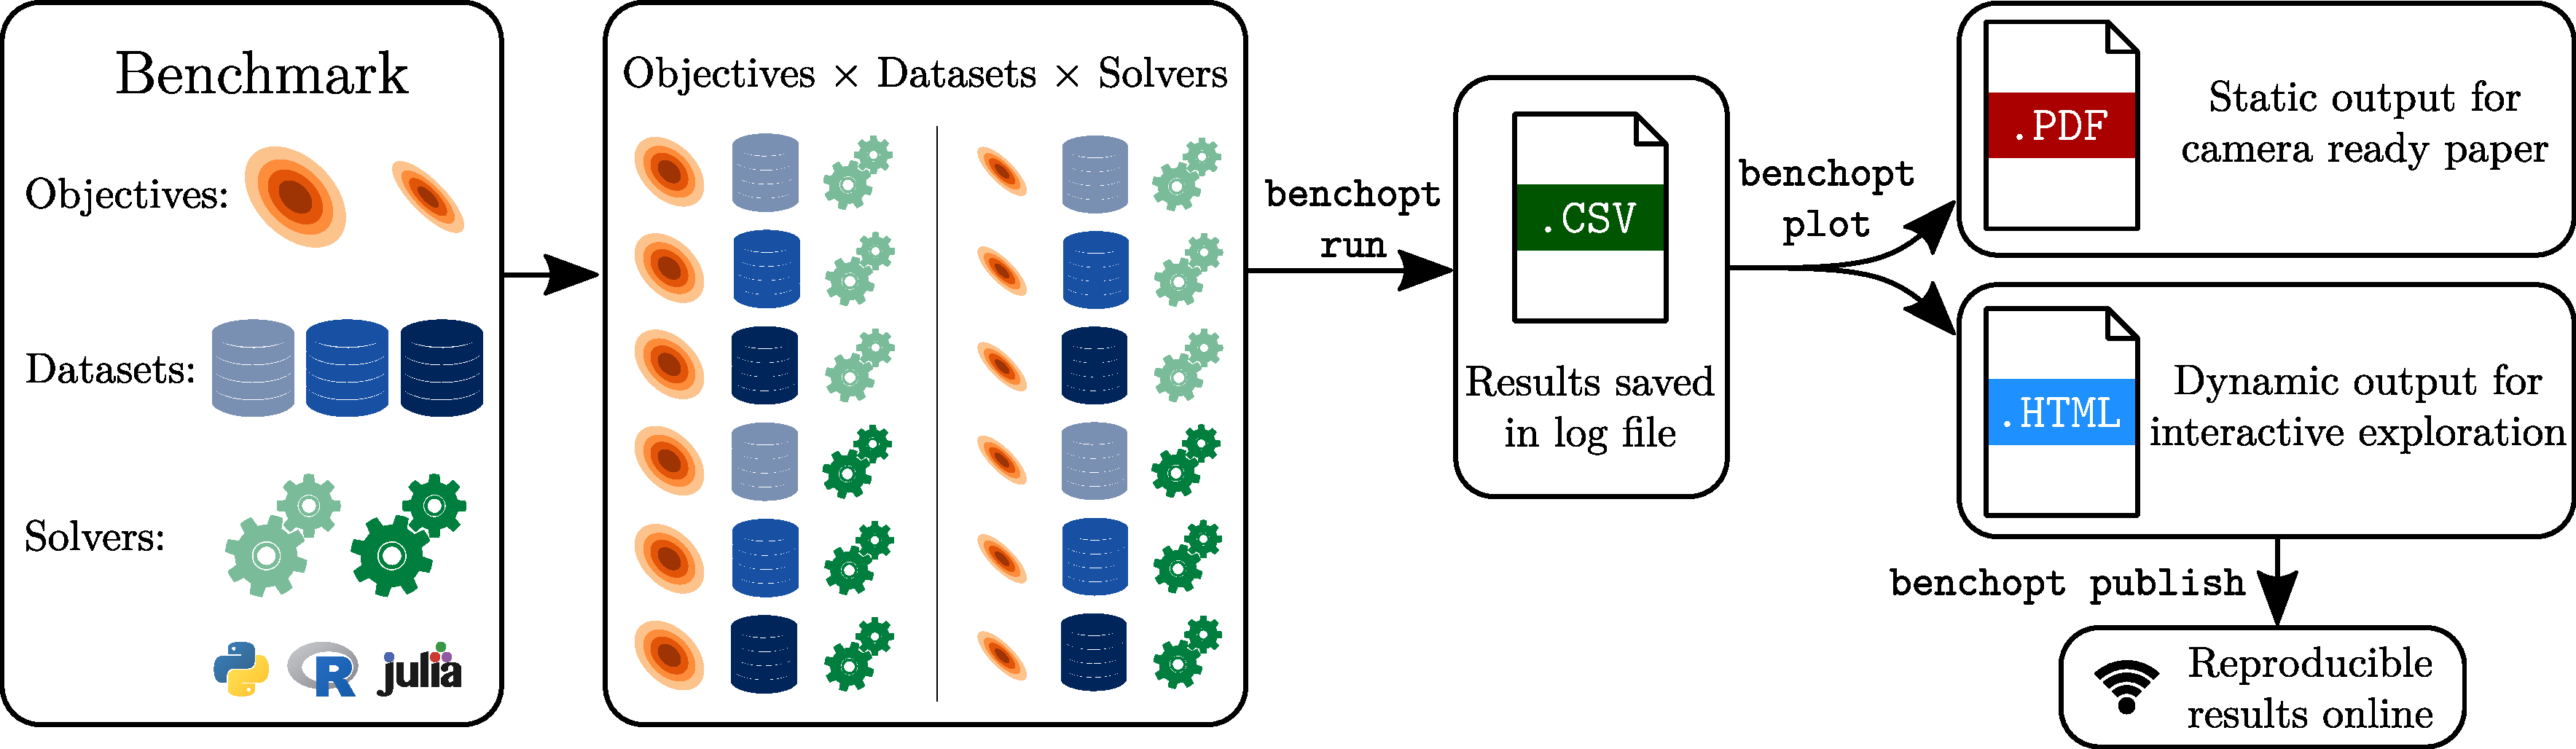
\includegraphics[width=\textwidth]{benchopt_schema_objectives_with_logos}

    \strongpoint{Each object can be parametrized so multiple scenario can be tested.}

    \vskip1.5em
    \textbf{Making tedious tasks easy:}\\[1em]
    \centering

    \myitem{} Sharing code
    \hskip3ex \myitem{} Adding methods
    \hskip3ex \myitem{} Exploring results\\[.5em]
    \myitem{} Varying hyperparameters
    \hskip3ex \myitem{} Running in Parallel
    \hskip3ex \myitem{} Caching\\[.5em]
    \hskip-4em\myitem{} \dots
}


%%%%%%%%%%%%%%%%%%%%%%%%%%%%%%%%%%%%%%%%%%%%%%%%%%%%%%%%%%%%%%%%%%%%%%%%%%%%%%%



\frame{
    \vskip2em
    {\centering
        \usebeamercolor[fg]{title}
        \usebeamerfont{title}
        \Huge \bf Thanks for your attention!\\[2em]}

    Slides are on my web page:\\[1em]
    \hskip5em\includegraphics[height=.8em]{website} tommoral.github.io
    \hskip4em 
\includegraphics[height=.8em]{twitter} @tomamoral

}


\end{document}
